\documentclass[aspectratio=169,10pt]{beamer}

% ---------------------------------------------------------------- packages --
\usepackage[utf8]{inputenc}
\usepackage[T1]{fontenc}
\usepackage{tikz}
\usetikzlibrary{arrows.meta,positioning,shapes.geometric,fit,backgrounds,calc}
\usepackage{amsmath,amssymb}
\usepackage{booktabs}
\usepackage{array}
\usepackage{colortbl}

% ------------------------------------------------------------------ theme ---
\usetheme{default}
\usecolortheme{default}
\setbeamertemplate{navigation symbols}{}
\setbeamertemplate{footline}[frame number]
\beamertemplatenavigationsymbolsempty

% palette (dataviz skill reference palette)
\definecolor{Ink}{HTML}{0B0B0B}
\definecolor{Ink2}{HTML}{52514E}
\definecolor{Muted}{HTML}{898781}
\definecolor{GridC}{HTML}{E1E0D9}
\definecolor{BaseC}{HTML}{C3C2B7}
\definecolor{SurfaceC}{HTML}{FCFCFB}
\definecolor{Cat1}{HTML}{2A78D6} % blue
\definecolor{Cat2}{HTML}{EB6834} % orange
\definecolor{Cat3}{HTML}{1BAF7A} % aqua
\definecolor{Cat4}{HTML}{EDA100} % yellow
\definecolor{Good}{HTML}{0CA30C}
\definecolor{WarningC}{HTML}{FAB219}
\definecolor{CriticalC}{HTML}{D03B3B}
\definecolor{SoftBlue}{HTML}{E8EDF6}
\definecolor{SoftGreen}{HTML}{E3F3EC}
\definecolor{SoftAmber}{HTML}{FDF1DA}
\definecolor{SoftRed}{HTML}{FAE3E2}

\setbeamercolor{normal text}{fg=Ink,bg=SurfaceC}
\setbeamercolor{background canvas}{bg=SurfaceC}
\setbeamercolor{frametitle}{fg=Ink,bg=SurfaceC}
\setbeamercolor{title}{fg=Ink}
\setbeamercolor{structure}{fg=Cat1}
\setbeamercolor{alerted text}{fg=CriticalC}
\setbeamercolor{page number in head/foot}{fg=Muted}
\setbeamerfont{frametitle}{series=\bfseries,size=\large}
\setbeamerfont{footline}{size=\tiny}

\setbeamertemplate{frametitle}{
  \vspace{2pt}
  {\usebeamerfont{frametitle}\usebeamercolor[fg]{frametitle}\insertframetitle}\\[-2pt]
  {\small\color{Ink2}\insertframesubtitle}
  \vspace{2pt}
  \color{GridC}\hrule height 0.6pt
}

\newcommand{\source}[1]{{\tiny\color{Muted} #1}}
\newcommand{\highlight}[1]{{\color{Cat1}\bfseries #1}}
\newcommand{\bad}[1]{{\color{CriticalC}\bfseries #1}}
\newcommand{\good}[1]{{\color{Good}\bfseries #1}}

\title{\textbf{Distribution-Aware Unionable Table Search}}
\subtitle{Pipeline schematic and experimental results on santosLarge, WDC, and the fairified benchmarks}
\author{DUTS experiment log}
\date{2026-08-12}

% ============================================================================
\begin{document}

% ---------------------------------------------------------------- title ----
\begin{frame}[plain]
  \begin{center}
    \vspace{0.6cm}
    {\Large\bfseries\color{Ink} Distribution-Aware Unionable Table Search}\\[6pt]
    {\large\color{Ink2} Pipeline schematic, short-circuits, and results on\\
     santosLarge and WDC (scalability), and the fairified benchmarks santos3, tusSmall3, tusLarge3 (quality)}\\[18pt]
    {\small\color{Muted} DUTS experiment log \quad\textbullet\quad 2026-08-12}
    \vspace{0.4cm}

    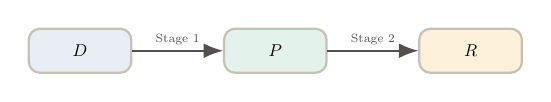
\begin{tikzpicture}[scale=0.62, every node/.style={scale=0.62}]
      \node[draw=BaseC, thick, rounded corners, fill=SoftBlue, minimum width=2.1cm, minimum height=0.9cm] (D) at (0,0) {$D$};
      \node[draw=BaseC, thick, rounded corners, fill=SoftGreen, minimum width=2.1cm, minimum height=0.9cm] (P) at (4,0) {$P$};
      \node[draw=BaseC, thick, rounded corners, fill=SoftAmber, minimum width=2.1cm, minimum height=0.9cm] (R) at (8,0) {$R$};
      \draw[-{Latex[length=2.5mm]}, Ink2, thick] (D) -- node[above,font=\scriptsize] {Stage 1} (P);
      \draw[-{Latex[length=2.5mm]}, Ink2, thick] (P) -- node[above,font=\scriptsize] {Stage 2} (R);
    \end{tikzpicture}
  \end{center}
\end{frame}

% -------------------------------------------------------------- agenda -----
\begin{frame}{Agenda}
\begin{columns}[T]
\begin{column}{0.48\textwidth}
\textbf{\color{Cat1}1. Pipeline schematic}
\begin{itemize}\small
  \item $D \to P \to R$ and the objectives at each stage
  \item Every short-circuit: where and why
\end{itemize}
\vspace{6pt}
\textbf{\color{Cat3}2. Fairified benchmarks -- quality}
\begin{itemize}\small
  \item santos3, tusSmall3, tusLarge3: one fair copy per (query, table) pair
  \item Feasibility, precision/recall, ideal recall, $\Sigma U$
  \item Which stages are bypassed; how often the LP pre-check is decisive
  \item Starmie baselines: pure Starmie, exhaustive swap, nested-loop swap
\end{itemize}
\end{column}
\begin{column}{0.48\textwidth}
\textbf{\color{Cat2}3. santosLarge -- scalability}
\begin{itemize}\small
  \item Why santosLarge, and choosing attributes/values to maximize $|D|$
  \item Choosing $F^\star$/$\delta$/$\tau$ to maximize reach
  \item The first configuration where $\alpha$ actually bites
  \item Index cost, per-stage timing at scale
\end{itemize}
\vspace{6pt}
\textbf{\color{Cat4}4. WDC -- 50.8M-table scalability}
\begin{itemize}\small
  \item Sampled tiers; maxD-style query selection replaces the old union-mode relaxation
  \item Choosing the $|D|$ threshold, a much larger $(k,\alpha)$ grid, and $F^\star/\delta/\tau$
  \item Final cohorts: 28 queries (\texttt{tier\_10k}), 30 queries (\texttt{tier\_100k}); \texttt{tier\_1m} pending
\end{itemize}
\vspace{6pt}
\textbf{\color{Ink}5. Takeaways}
\end{column}
\end{columns}
\end{frame}

% ============================================================================
\section{Pipeline schematic}
% ============================================================================
\begin{frame}{The two-stage pipeline}{$D \to P \to R$, and what each stage optimizes}
\begin{center}
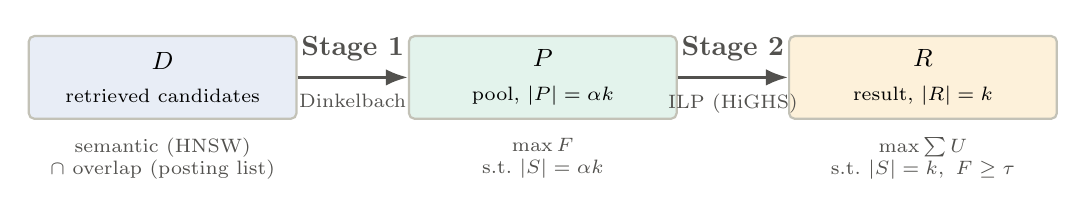
\begin{tikzpicture}[
  node distance=8mm and 14mm,
  box/.style={draw=BaseC, thick, rounded corners=2pt, minimum height=1.05cm, align=center, font=\small},
  stage/.style={box, fill=SoftBlue, minimum width=3.4cm},
  obj/.style={font=\scriptsize, color=Ink2, align=center},
  arr/.style={-{Latex[length=2.8mm]}, Ink2, line width=1pt}
]
\node[stage] (D) {$D$\\[1pt]{\scriptsize retrieved candidates}};
\node[stage, fill=SoftGreen, right=of D] (P) {$P$\\[1pt]{\scriptsize pool, $|P|=\alpha k$}};
\node[stage, fill=SoftAmber, right=of P] (R) {$R$\\[1pt]{\scriptsize result, $|R|=k$}};

\draw[arr] (D) -- node[above=2pt]{\textbf{Stage 1}} node[below=2pt]{\scriptsize Dinkelbach} (P);
\draw[arr] (P) -- node[above=2pt]{\textbf{Stage 2}} node[below=2pt]{\scriptsize ILP (HiGHS)} (R);

\node[obj, below=3pt of D] {semantic (HNSW)\\ $\cap$ overlap (posting list)};
\node[obj, below=3pt of P] {$\max F$\\ s.t.\ $|S|=\alpha k$};
\node[obj, below=3pt of R] {$\max \sum U$\\ s.t.\ $|S|=k,\ F\geq\tau$};
\end{tikzpicture}

\vspace{6pt}
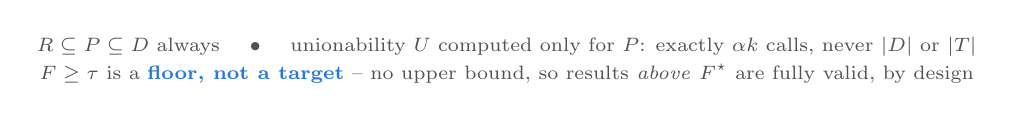
\begin{tikzpicture}[scale=0.9]
\node[font=\scriptsize, color=Ink2, align=center] {$R \subseteq P \subseteq D$ always $\quad\bullet\quad$ unionability $U$ computed only for $P$: exactly $\alpha k$ calls, never $|D|$ or $|T|$\\[2pt]
$F\geq\tau$ is a \highlight{floor, not a target} -- no upper bound, so results \emph{above} $F^\star$ are fully valid, by design};
\end{tikzpicture}
\end{center}
\end{frame}

\begin{frame}{The full process -- with every short-circuit}{Where an instance can exit early, and why}
\begin{center}
\resizebox{!}{0.83\textheight}{%
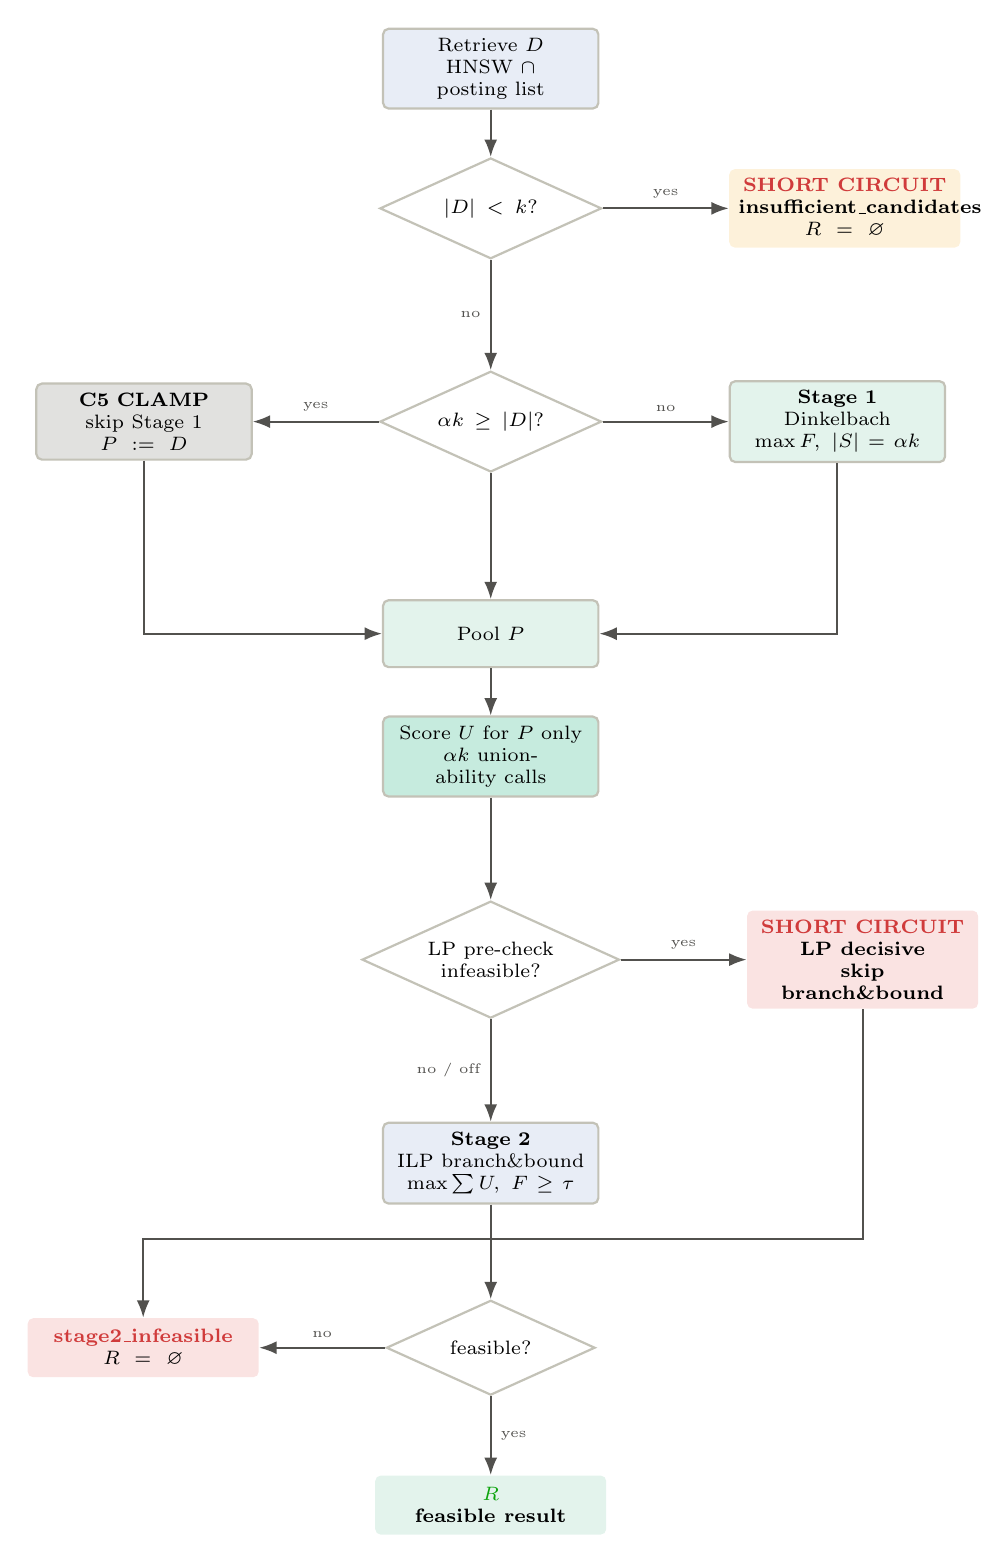
\begin{tikzpicture}[
  node distance=6mm and 10mm,
  box/.style={draw=BaseC, thick, rounded corners=2pt, minimum height=0.85cm, align=center, font=\scriptsize, text width=2.5cm},
  dec/.style={draw=BaseC, thick, diamond, aspect=2.2, align=center, font=\scriptsize, inner sep=1pt, text width=2.05cm},
  outcome/.style={draw=none, rounded corners=2pt, minimum height=0.75cm, align=center, font=\scriptsize\bfseries, text width=2.7cm},
  arr/.style={-{Latex[length=2.2mm]}, Ink2, line width=0.7pt},
  yesno/.style={font=\tiny, color=Ink2}
]
% retrieval
\node[box, fill=SoftBlue] (retr) {Retrieve $D$\\{\scriptsize HNSW $\cap$ posting list}};
\node[dec, below=of retr] (chk1) {$|D|<k$?};
\node[outcome, fill=SoftAmber, right=16mm of chk1] (sc1) {\bad{SHORT CIRCUIT}\\insufficient\_candidates\\$R=\varnothing$};

\node[dec, below=14mm of chk1] (chk2) {$\alpha k \geq |D|$?};
\node[box, fill=Muted!25, left=16mm of chk2] (clamp) {\textbf{C5 CLAMP}\\skip Stage 1\\$P := D$};
\node[box, fill=SoftGreen, right=16mm of chk2] (s1) {\textbf{Stage 1}\\Dinkelbach\\$\max F,\ |S|=\alpha k$};

\node[box, fill=SoftGreen, below=16mm of chk2] (pool) {Pool $P$};
\node[box, fill=Cat3!25, below=of pool] (score) {Score $U$ for $P$ only\\{\scriptsize $\alpha k$ unionability calls}};

\node[dec, below=13mm of score] (chk3) {LP pre-check\\infeasible?};
\node[outcome, fill=SoftRed, right=16mm of chk3] (sc2) {\bad{SHORT CIRCUIT}\\LP decisive\\skip branch\&bound};
\node[box, fill=SoftBlue, below=13mm of chk3] (ilp) {\textbf{Stage 2}\\ILP branch\&bound\\$\max \sum U,\ F\geq\tau$};

\node[dec, below=12mm of ilp] (chk4) {feasible?};
\node[outcome, fill=SoftRed, left=16mm of chk4] (sc3) {\bad{stage2\_infeasible}\\$R=\varnothing$};
\node[outcome, fill=SoftGreen, below=10mm of chk4] (done) {\good{$R$}\\feasible result};

% arrows
\draw[arr] (retr) -- (chk1);
\draw[arr] (chk1) -- node[yesno,above]{yes} (sc1);
\draw[arr] (chk1) -- node[yesno,left]{no} (chk2);
\draw[arr] (chk2) -- node[yesno,above]{yes} (clamp);
\draw[arr] (chk2) -- node[yesno,above]{no} (s1);
\draw[arr] (clamp) |- (pool);
\draw[arr] (s1) |- (pool);
\draw[arr] (chk2) -- (pool);
\draw[arr] (pool) -- (score);
\draw[arr] (score) -- (chk3);
\draw[arr] (chk3) -- node[yesno,above]{yes} (sc2);
\draw[arr] (chk3) -- node[yesno,left]{no / off} (ilp);
\draw[arr] (sc2) |- ($(sc3.north)+(0,10mm)$) -- (sc3);
\draw[arr] (ilp) -- (chk4);
\draw[arr] (chk4) -- node[yesno,above]{no} (sc3);
\draw[arr] (chk4) -- node[yesno,right]{yes} (done);
\end{tikzpicture}}
\end{center}
\end{frame}

\begin{frame}{Short-circuits -- what each one means}
\small
\begin{tabular}{@{}p{3.1cm}p{5.1cm}p{3.6cm}@{}}
\toprule
\textbf{Short-circuit} & \textbf{Condition} & \textbf{Cost avoided} \\
\midrule
\cellcolor{SoftAmber!60}\texttt{insufficient\_\allowbreak candidates} & $|D|<k$ before Stage 1 even starts & Stage 1, scoring, Stage 2 -- all of it \\[4pt]
\cellcolor{Muted!25}C5 clamp & $\alpha k \geq |D|$, so $P{:=}D$ & Dinkelbach never runs (\emph{not} run-and-discarded) \\[4pt]
\cellcolor{SoftRed!70}LP pre-check decisive & LP relaxation already infeasible & ILP branch-and-bound \\[4pt]
\cellcolor{SoftRed!70}\texttt{stage2\_\allowbreak infeasible} & ILP proves no $k$-subset of $P$ reaches $\tau$ & -- (this is the answer) \\
\bottomrule
\end{tabular}
\vspace{8pt}

{\footnotesize\color{Ink2} The C4 feasibility certificate (a would-be short-circuit \emph{before} Stage 1, splitting \texttt{insufficient\_candidates} from an "intrinsically infeasible" cause) was removed from this pipeline entirely -- \texttt{stage2\_infeasible} is now the only post-retrieval failure label.}
\end{frame}

% ============================================================================
\section{Fairified benchmarks -- santos3, tusSmall3, tusLarge3}

\begin{frame}{Fairified benchmarks: setup and what is reported}{same pipeline, same metrics on all three -- $F^*{=}0.4$, $\delta{=}0.1$ ($\tau{=}0.3$), $top\_n{=}1000$}
\small
\begin{center}
\setlength{\tabcolsep}{5pt}
\begin{tabular}{lrrr}
\toprule
 & santos3 & tusSmall3 & tusLarge3 \\
\midrule
fair queries & 48 & 92 & 142 \\
datalake tables (originals + fair copies) & 999 & 9,178 & 18,309 \\
mean ground truth tables / query & 28.1 & 852.7 & 626.7 \\
own fair copies / query (min / mean) & 1 / 11.0 & 16 / 85.9 & 27 / 100.0 \\
mean $|D|$ & 25.5 & 122.5 & 90.5 \\
\bottomrule
\end{tabular}
\end{center}
\vspace{4pt}
\begin{itemize}\setlength\itemsep{2pt}
\item Grid: $k\in\{5,10,20\}\times\alpha\in\{10,5\}$; real pinned-match $U$ ($\sigma{=}0.6$).
\item \textbf{Precision, recall, $\Sigma U$ and $F_R$ are means over all queries; a failed query (empty result) counts 0.} \textbf{Ideal recall} is over all queries and is identical for every method.
\item Also reported: feasible queries, \textbf{bypassed stages} and LP pre-check decisions.
\end{itemize}
{\footnotesize\color{Muted} All three are built the same way: one fair copy per (query, table) pair, ratio $\ge0.4$ for the query's value, matched by column name. A table that cannot be augmented for a query is removed from \emph{that query's} ground truth (and from the datalake if it fails for every query), so every ground-truth table has a fair version for its query. The original table and each fair copy are separate unionable tables (both count as hits in precision/recall; the original may not carry enough of the value to reach $\tau$). Ground truth includes every copy of a unionable table. Protected value matched with numeric spelling variants (\texttt{4}/\texttt{4.0}). Details: \texttt{fair3-report.md}.}
\end{frame}

% ---- top_n=1000 quality
\begin{frame}{Fairified benchmarks: Quality of the fair result R}{top\_n$=1000$, $F^*{=}0.4$, $\delta{=}0.1$, $\alpha\in\{10,5\}\times k\in\{5,10,20\}$}
\scriptsize
\begin{center}
\setlength{\tabcolsep}{2.5pt}
\resizebox{\ifdim\width>\textwidth\textwidth\else\width\fi}{!}{%
\begin{tabular}{lrrrrrrrr}
\toprule
bench & $\alpha$ & k & feasible & precision@R & recall@R & ideal recall & mean $\Sigma$U & mean F$_R$ \\
\midrule
\texttt{santos3} & 10 & 5 & 42/48 & 0.875 & 0.1769 & 0.2984 & 52.8 & 0.388 \\
\texttt{santos3} & 10 & 10 & 39/48 & 0.810 & 0.3005 & 0.4736 & 96.0 & 0.355 \\
\texttt{santos3} & 10 & 20 & 26/48 & 0.520 & 0.3352 & 0.7299 & 111.7 & 0.239 \\
\texttt{santos3} & 5 & 5 & 42/48 & 0.846 & 0.1723 & 0.2984 & 51.2 & 0.405 \\
\texttt{santos3} & 5 & 10 & 39/48 & 0.810 & 0.3005 & 0.4736 & 95.9 & 0.360 \\
\texttt{santos3} & 5 & 20 & 26/48 & 0.520 & 0.3352 & 0.7299 & 111.7 & 0.239 \\
\texttt{tusSmall3} & 10 & 5 & 89/92 & 0.933 & 0.0100 & 0.0105 & 46.3 & 0.364 \\
\texttt{tusSmall3} & 10 & 10 & 84/92 & 0.890 & 0.0197 & 0.0211 & 85.6 & 0.297 \\
\texttt{tusSmall3} & 10 & 20 & 65/92 & 0.678 & 0.0347 & 0.0421 & 114.1 & 0.221 \\
\texttt{tusSmall3} & 5 & 5 & 89/92 & 0.920 & 0.0098 & 0.0105 & 46.0 & 0.393 \\
\texttt{tusSmall3} & 5 & 10 & 84/92 & 0.864 & 0.0192 & 0.0211 & 85.1 & 0.338 \\
\texttt{tusSmall3} & 5 & 20 & 65/92 & 0.665 & 0.0339 & 0.0421 & 113.6 & 0.232 \\
\texttt{tusLarge3} & 10 & 5 & 133/142 & 0.790 & 0.0101 & 0.0125 & 50.3 & 0.348 \\
\texttt{tusLarge3} & 10 & 10 & 122/142 & 0.715 & 0.0190 & 0.0249 & 88.9 & 0.288 \\
\texttt{tusLarge3} & 10 & 20 & 93/142 & 0.526 & 0.0291 & 0.0498 & 121.5 & 0.208 \\
\texttt{tusLarge3} & 5 & 5 & 133/142 & 0.782 & 0.0099 & 0.0125 & 49.8 & 0.375 \\
\texttt{tusLarge3} & 5 & 10 & 122/142 & 0.704 & 0.0184 & 0.0249 & 88.2 & 0.308 \\
\texttt{tusLarge3} & 5 & 20 & 93/142 & 0.518 & 0.0283 & 0.0498 & 120.5 & 0.218 \\
\bottomrule
\end{tabular}}
\end{center}
\end{frame}

\begin{frame}{What the quality table shows}{findings in plain words -- $\alpha{=}10$, $top\_n{=}1000$}
\small
\begin{itemize}\setlength\itemsep{4pt}
\item \highlight{Most queries get a fair answer.} Feasible queries ($k{=}5/10/20$): santos3 $42/39/26$ of 48, tusSmall3 $89/84/65$ of 92, tusLarge3 $133/122/93$ of 142. Feasible means $k$ tables whose union with the query has at least $30\%$ rows with the protected value.
\item \highlight{Precision and recall are means over all queries; a failed query counts 0.} precision@R: santos3 $0.88/0.81/0.52$, tusSmall3 $0.93/0.89/0.68$, tusLarge3 $0.79/0.72/0.53$. They fall with $k$ mainly because more queries fail.
\item \highlight{Recall stays below the ideal recall} (the best possible with $k$ tables, the same for every method): santos3 $0.18/0.30/0.34$ vs $0.30/0.47/0.73$, tusSmall3 $0.010/0.020/0.035$ vs $0.011/0.021/0.042$, tusLarge3 $0.010/0.019/0.029$ vs $0.012/0.025/0.050$. The gap is widest where many queries fail (santos3, $k{=}20$: 26 of 48 feasible).
\item \highlight{The fairness target is met} where an answer exists: among the feasible queries $F_R\ge0.31$ ($\tau{=}0.30$), about $0.44$ on santos3 and $0.31$--$0.41$ on TUS. In the table $\Sigma U$ and $F_R$ are means over \textbf{all} queries with a failed query counting 0, so they are lower where queries fail.
\end{itemize}
\vspace{2pt}
{\footnotesize\color{Muted} Example: tusSmall3, $\alpha{=}10$, $k{=}5$: 89 of 92 feasible, precision $0.933$, recall $0.0100$ vs ideal $0.0105$.}
\end{frame}

% ---- top_n=1000 stages
\begin{frame}{Fairified benchmarks: Stage bypasses, LP pre-check and feasibility}{top\_n$=1000$, $F^*{=}0.4$, $\delta{=}0.1$, $\alpha\in\{10,5\}\times k\in\{5,10,20\}$}
\scriptsize
\begin{center}
\setlength{\tabcolsep}{2.5pt}
\begin{tabular}{lrrrrrrrrrrr}
\toprule
bench & $\alpha$ & $k$ & $|D|$ & $|D|{<}k$ & S1 skip & S1 ran & LP dec. & MILP ran & feasible & $\ge k$ own & feas.\ among \\
\midrule
\texttt{santos3} & 10 & 5 & 25.5 & 4 & 40 & 4 & 2 & 42 & 42/48 & 39 & 39/39 \\
\texttt{santos3} & 10 & 10 & 25.5 & 7 & 41 & 0 & 2 & 39 & 39/48 & 36 & 35/36 \\
\texttt{santos3} & 10 & 20 & 25.5 & 20 & 28 & 0 & 2 & 26 & 26/48 & 3 & 3/3 \\
\texttt{santos3} & 5 & 5 & 25.5 & 4 & 27 & 17 & 2 & 42 & 42/48 & 39 & 39/39 \\
\texttt{santos3} & 5 & 10 & 25.5 & 7 & 37 & 4 & 2 & 39 & 39/48 & 36 & 35/36 \\
\texttt{santos3} & 5 & 20 & 25.5 & 20 & 28 & 0 & 2 & 26 & 26/48 & 3 & 3/3 \\
\texttt{tusSmall3} & 10 & 5 & 122.5 & 0 & 11 & 81 & 3 & 89 & 89/92 & 92 & 89/92 \\
\texttt{tusSmall3} & 10 & 10 & 122.5 & 1 & 42 & 49 & 7 & 84 & 84/92 & 92 & 84/92 \\
\texttt{tusSmall3} & 10 & 20 & 122.5 & 2 & 77 & 13 & 25 & 65 & 65/92 & 85 & 58/85 \\
\texttt{tusSmall3} & 5 & 5 & 122.5 & 0 & 3 & 89 & 3 & 89 & 89/92 & 92 & 89/92 \\
\texttt{tusSmall3} & 5 & 10 & 122.5 & 1 & 10 & 81 & 7 & 84 & 84/92 & 92 & 84/92 \\
\texttt{tusSmall3} & 5 & 20 & 122.5 & 2 & 41 & 49 & 25 & 65 & 65/92 & 85 & 58/85 \\
\texttt{tusLarge3} & 10 & 5 & 90.5 & 6 & 34 & 102 & 3 & 133 & 133/142 & 142 & 133/142 \\
\texttt{tusLarge3} & 10 & 10 & 90.5 & 10 & 76 & 56 & 10 & 122 & 122/142 & 142 & 122/142 \\
\texttt{tusLarge3} & 10 & 20 & 90.5 & 15 & 119 & 8 & 34 & 93 & 93/142 & 142 & 93/142 \\
\texttt{tusLarge3} & 5 & 5 & 90.5 & 6 & 10 & 126 & 3 & 133 & 133/142 & 142 & 133/142 \\
\texttt{tusLarge3} & 5 & 10 & 90.5 & 10 & 30 & 102 & 10 & 122 & 122/142 & 142 & 122/142 \\
\texttt{tusLarge3} & 5 & 20 & 90.5 & 15 & 71 & 56 & 34 & 93 & 93/142 & 142 & 93/142 \\
\bottomrule
\end{tabular}
\end{center}
\end{frame}

\begin{frame}{What the stage table shows}{how each query ends, and which stages were skipped -- $\alpha{=}10$, $top\_n{=}1000$}
\small
\begin{itemize}\setlength\itemsep{4pt}
\item Every query ends one of three ways: \highlight{$|D|<k$} (too few candidates -- Stage 1 and 2 skipped), \highlight{LP decisive} (the LP proves no $k$ tables reach $F\ge0.3$ -- MILP skipped) or \highlight{MILP ran} (feasible; the MILP never failed after a feasible LP).
\item \highlight{santos3:} the failures are mostly too few candidates: $|D|{<}k$ for 4 / 7 / 20 of the 6 / 9 / 22 infeasible queries at $k{=}5/10/20$. Own copies are a sufficient, not a necessary, condition: only 3 queries have $\ge20$ own fair copies, yet 26 are feasible at $k{=}20$, because the kept original tables and other queries' copies fill the slots. Among queries with $\ge k$ own copies: $39/39$, $35/36$, $3/3$.
\item \highlight{TUS:} every query has at least $k$ own copies for $k\le10$, yet $3$--$20$ queries per row are infeasible -- retrieval did not bring enough of them into $D$ (next slides).
\item \highlight{Stage 1 is bypassed} ($P{=}D$) for most santos3 queries and for most TUS queries at $k{=}20$ (77/92, 119/142); at $k{=}5$ it runs for most TUS queries (81/92, 102/142). The LP pre-check is decisive for $2$--$34$ queries per row, each skipping a MILP call.
\end{itemize}
\vspace{2pt}
{\footnotesize\color{Muted} Columns: $|D|$ mean candidates; $|D|{<}k$ both stages skipped; S1 skip Stage 1 bypassed ($P{=}D$); S1 ran; LP dec.\ LP pre-check decisive (MILP skipped); MILP ran; $\ge k$ own queries with at least $k$ own fair copies; feas.\ among feasible among those.}
\vspace{2pt}
{\footnotesize\color{Muted} Example: tusSmall3, $\alpha{=}10$, $k{=}20$: $92 = 2\ (|D|{<}k) + 25\ (\text{LP infeasible}) + 65\ (\text{feasible})$. The optimizer cannot fix these failures: it only chooses inside $D$.}
\end{frame}

% ---- top_n=1000 dpr
\begin{frame}{Fairified benchmarks: Precision and recall at D, P and R}{top\_n$=1000$, $F^*{=}0.4$, $\delta{=}0.1$, $\alpha\in\{10,5\}\times k\in\{5,10,20\}$}
\scriptsize
\begin{center}
\setlength{\tabcolsep}{2.5pt}
\resizebox{\ifdim\width>\textwidth\textwidth\else\width\fi}{!}{%
\begin{tabular}{lrrrrrrrr}
\toprule
bench & $\alpha$ & k & prec@D & rec@D & prec@P & rec@P & prec@R & rec@R \\
\midrule
\texttt{santos3} & 10 & 5 & 0.899 & 0.8216 & 0.813 & 0.7266 & 0.875 & 0.1769 \\
\texttt{santos3} & 10 & 10 & 0.899 & 0.8216 & 0.769 & 0.6910 & 0.810 & 0.3005 \\
\texttt{santos3} & 10 & 20 & 0.899 & 0.8216 & 0.516 & 0.5233 & 0.520 & 0.3352 \\
\texttt{santos3} & 5 & 5 & 0.899 & 0.8216 & 0.799 & 0.6100 & 0.846 & 0.1723 \\
\texttt{santos3} & 5 & 10 & 0.899 & 0.8216 & 0.766 & 0.6724 & 0.810 & 0.3005 \\
\texttt{santos3} & 5 & 20 & 0.899 & 0.8216 & 0.516 & 0.5233 & 0.520 & 0.3352 \\
\texttt{tusSmall3} & 10 & 5 & 0.934 & 0.2585 & 0.923 & 0.0953 & 0.933 & 0.0100 \\
\texttt{tusSmall3} & 10 & 10 & 0.934 & 0.2585 & 0.916 & 0.1729 & 0.890 & 0.0197 \\
\texttt{tusSmall3} & 10 & 20 & 0.934 & 0.2585 & 0.912 & 0.2352 & 0.678 & 0.0347 \\
\texttt{tusSmall3} & 5 & 5 & 0.934 & 0.2585 & 0.928 & 0.0487 & 0.920 & 0.0098 \\
\texttt{tusSmall3} & 5 & 10 & 0.934 & 0.2585 & 0.913 & 0.0952 & 0.864 & 0.0192 \\
\texttt{tusSmall3} & 5 & 20 & 0.934 & 0.2585 & 0.905 & 0.1728 & 0.665 & 0.0339 \\
\texttt{tusLarge3} & 10 & 5 & 0.746 & 0.1570 & 0.723 & 0.0767 & 0.790 & 0.0101 \\
\texttt{tusLarge3} & 10 & 10 & 0.746 & 0.1570 & 0.694 & 0.1226 & 0.715 & 0.0190 \\
\texttt{tusLarge3} & 10 & 20 & 0.746 & 0.1570 & 0.657 & 0.1456 & 0.526 & 0.0291 \\
\texttt{tusLarge3} & 5 & 5 & 0.746 & 0.1570 & 0.744 & 0.0444 & 0.782 & 0.0099 \\
\texttt{tusLarge3} & 5 & 10 & 0.746 & 0.1570 & 0.696 & 0.0764 & 0.704 & 0.0184 \\
\texttt{tusLarge3} & 5 & 20 & 0.746 & 0.1570 & 0.659 & 0.1211 & 0.518 & 0.0283 \\
\bottomrule
\end{tabular}}
\end{center}
\end{frame}

\begin{frame}{What the precision/recall table shows}{the same measures at $D$, $P$ and $R$, all queries -- $\alpha{=}10$, $top\_n{=}1000$}
\small
\begin{itemize}\setlength\itemsep{4pt}
\item $D$: tables retrieved (before any selection). $P$: the pool of $\alpha k$ tables chosen by Stage 1. $R$: the final $k$ tables. An empty or missing set (no pool because $|D|{<}k$, or no result because the query failed) counts 0.
\item \highlight{The retrieved set is mostly unionable:} precision@D $0.90$ (santos3), $0.93$ (tusSmall3), $0.75$ (tusLarge3); recall@D $0.82/0.26/0.16$.
\item \highlight{Precision at $P$ and $R$ stays close to $D$ where queries succeed,} and drops at large $k$ because queries fail: santos3 precision@R $0.88/0.81/0.52$ (only 26 of 48 queries have a result at $k{=}20$).
\item \highlight{Recall falls from $D$ to $R$ because the sets shrink} ($D$ holds $\sim$25 / 120 / 90 tables, $R$ holds $k$) and because failed queries count 0.
\end{itemize}
\vspace{2pt}
{\footnotesize\color{Muted} Example: tusSmall3, $\alpha{=}10$, $k{=}5$: precision $0.934\to0.923\to0.933$ and recall $0.259\to0.095\to0.0100$ at $D\to P\to R$. Precision/recall at $D$ do not depend on $k$ or $\alpha$.}
\end{frame}

\begin{frame}{Why some queries stay infeasible: own fair copies in $D$}{$top\_n{=}1000$ -- each query has its own fair copies (ratio $\ge0.4$ for its value) in the datalake}
\small
\begin{center}
\setlength{\tabcolsep}{4pt}
\begin{tabular}{lrrrrr}
\toprule
benchmark & mean $|D|$ & own copies in $D$ & own copies in datalake & ratio over $D$ & ratio, own copies in $D$ \\
\midrule
\texttt{santos3} & 25.5 & 9.9 & 11.0 & 0.372 & 0.485 \\
\texttt{tusSmall3} & 122.4 & 17.1 & 85.9 & 0.152 & 0.396 \\
\texttt{tusLarge3} & 83.8 & 13.6 & 100.0 & 0.173 & 0.386 \\
\bottomrule
\end{tabular}
\end{center}
\vspace{4pt}
\begin{itemize}\setlength\itemsep{3pt}
\item \highlight{santos3:} retrieval brings almost all of the query's own copies into $D$ (9.9 of 11.0) and the ratio over $D$ ($0.37$) is above $\tau{=}0.3$; the failures come mostly from queries with fewer than $k$ candidates.
\item \highlight{TUS:} only $\sim$17 of $\sim$86 (tusSmall3) and $\sim$14 of 100 (tusLarge3) own copies reach $D$; the ratio over all of $D$ ($0.15$--$0.17$) is below $\tau$. Copies of one table have nearly identical vectors, so the $top\_n$ window fills with originals and with copies made for \emph{other} queries, where the query's value is rare. 9 of 142 tusLarge3 queries get none.
\item Retrieval is not fairness-aware and the optimizer only sees $D$: these failures are a retrieval limit, and the MILP never failed.
\end{itemize}
{\footnotesize\color{Muted} Separate run of the same code (own HNSW build), so $|D|$ differs slightly from the tables. Details: \texttt{fair3-report.md}.}
\end{frame}

\section{Starmie baselines -- pure Starmie, exhaustive swap, nested-loop swap}

\begin{frame}{Starmie baselines: what was run}{same fair queries, datalake and ground truth as the DUTS tables -- no timings reported}
\footnotesize
\begin{itemize}\setlength\itemsep{3pt}
\item \highlight{Pure Starmie:} the $N$ nearest columns of every query column give the candidates; each is scored by bipartite column matching; the top-$k$ is returned. No protected attribute is used.
\item \highlight{Exhaustive swap (no filtering):} candidates are scored with the protected column \emph{pinned} in the matching; if the initial top-$k$ has $F<\tau$, violating tables are swapped out for the best replacement, trying \emph{every} candidate.
\item \highlight{Nested-loop swap (winnow filtering):} the same swap, but the candidates are first pruned by a dominance filter (a candidate is dropped if another has more protected rows, fewer other rows and at least as good unionability).
\item Fixed for all three: $N{=}1000$, $\sigma{=}0.6$, $F^*{=}0.4$, $\delta{=}0.1$ ($\tau{=}0.3$), $k\in\{5,10,20\}$, on santos3 (48 queries), tusSmall3 (92), tusLarge3 (142).
\item \textbf{Metrics, recomputed by our code as for DUTS.} Precision, recall and ideal recall are means over \textbf{all} queries. For the two swap methods an infeasible query (not exactly $k$ tables with $F\ge\tau$) counts 0 for precision, recall, $\Sigma U$ and $F_R$. \textbf{Pure Starmie is scored on what it returns, regardless of $\tau$}, with the number of queries that reached $\tau$ shown beside it; its precision, recall, $\Sigma U$ and $F$ are over all queries.
\end{itemize}
{\footnotesize\color{Muted} The baselines are Starmie's own code (\texttt{HNSWSearcher\_Fair}), run unmodified except for the three changes listed on the next slide. Because pure Starmie is not zeroed when it misses $\tau$, its precision and recall count unfair lists and are not directly comparable with the swap methods'.}
\end{frame}

\begin{frame}{Starmie baselines: defaults and changes}{taken from the Starmie code, not chosen by us}
\small
\begin{itemize}\setlength\itemsep{3pt}\footnotesize
\item \highlight{Index:} HNSW, cosine, $M{=}32$, $ef_{construction}{=}100$, $ef{=}10$ (a query with $N{=}1000$ uses $\max(ef,N)$); tables shuffled with seed 42 at scale 1.0.
\item \highlight{Matching:} an edge counts if cosine $>\sigma$. We use $\sigma{=}0.6$, as DUTS; Starmie's own default for these benchmarks is $0.7$.
\item \highlight{Dominance rules} of the nested-loop filter: the bundled \texttt{preference\_config.json} (protected count, non-protected count, unionability score), unchanged.
\item \highlight{Swap algorithms:} default removal and replacement order; no parameters were set.
\item \highlight{$F$:} Starmie's \texttt{compute\_F} over the benchmark's \texttt{metadata\_combined.pkl}: any column counts as categorical (no $\theta_{cat}{=}50$ limit); a table adds rows only if its protected column aligns in the constrained matching; the query is included. Pure Starmie is scored after the fact with the same alignment.
\item \highlight{Our three changes:} (1) the protected value is matched with its numeric spelling variants (\texttt{4}/\texttt{4.0}), as in the DUTS runs; (2) the raw datalake is not loaded into memory and the metadata pickle is not rewritten; (3) the index is written to a scratch folder.
\item \highlight{Metrics:} recomputed from the returned lists (Starmie's own script averages precision only over queries with $|gt|\ge k$ and uses an uncapped ideal recall, so it is not comparable).
\item \highlight{$\Sigma U$:} Starmie's matching score of the returned tables; it equals the DUTS pinned-match score in all but 20 of 2{,}538 rows.
\end{itemize}
\end{frame}

% ---- starmie main
\begin{frame}{Pure Starmie (no fairification): results}{$N{=}1000$, $\sigma{=}0.6$, $F^*{=}0.4$, $\delta{=}0.1$}
\scriptsize
\begin{center}
\setlength{\tabcolsep}{2.5pt}
\resizebox{\ifdim\width>\textwidth\textwidth\else\width\fi}{!}{%
\begin{tabular}{lrrrrrrr}
\toprule
bench & k & reached $\tau$ & precision & recall & ideal recall & mean $\Sigma$U & mean $F$ \\
\midrule
\texttt{santos3} & 5 & 21/48 & 0.888 & 0.2772 & 0.2984 & 60.0 & 0.337 \\
\texttt{santos3} & 10 & 12/48 & 0.829 & 0.4216 & 0.4736 & 115.7 & 0.269 \\
\texttt{santos3} & 20 & 9/48 & 0.752 & 0.6516 & 0.7299 & 220.0 & 0.206 \\
\texttt{tusSmall3} & 5 & 7/92 & 0.900 & 0.0098 & 0.0105 & 50.2 & 0.161 \\
\texttt{tusSmall3} & 10 & 5/92 & 0.886 & 0.0195 & 0.0211 & 100.1 & 0.126 \\
\texttt{tusSmall3} & 20 & 1/92 & 0.843 & 0.0358 & 0.0421 & 198.5 & 0.094 \\
\texttt{tusLarge3} & 5 & 22/142 & 0.792 & 0.0099 & 0.0125 & 55.9 & 0.183 \\
\texttt{tusLarge3} & 10 & 13/142 & 0.769 & 0.0191 & 0.0249 & 111.0 & 0.143 \\
\texttt{tusLarge3} & 20 & 8/142 & 0.713 & 0.0348 & 0.0498 & 219.4 & 0.108 \\
\bottomrule
\end{tabular}}
\end{center}
\vspace{2pt}
{\footnotesize\color{Muted} Pure Starmie is scored on the list it returns, \emph{regardless of $\tau$}: precision, recall, ideal recall, $\Sigma U$ and $F$ are means over \textbf{all} queries. \emph{reached $\tau$}: queries whose unfair top-$k$ has $F\ge\tau{=}0.3$.}
\end{frame}

\begin{frame}{What the pure Starmie table shows}{findings in plain words -- all queries, as returned, regardless of $\tau$}
\small
\begin{itemize}\setlength\itemsep{4pt}
\item \highlight{The unfair top-$k$ rarely meets the fairness target.} It has $F\ge0.3$ for only santos3 $21/12/9$ of 48, tusSmall3 $7/5/1$ of 92, tusLarge3 $22/13/8$ of 142 queries ($k{=}5/10/20$).
\item \highlight{It gets worse as $k$ grows.} Mean $F$ over all queries: santos3 $0.34/0.27/0.21$, tusSmall3 $0.16/0.13/0.09$, tusLarge3 $0.18/0.14/0.11$; $\Sigma U$ grows with $k$ ($60/116/220$ on santos3).
\item \highlight{Precision over all queries:} $0.89/0.83/0.75$ (santos3), $0.90/0.89/0.84$ (tusSmall3), $0.79/0.77/0.71$ (tusLarge3).
\item \highlight{Recall vs ideal recall:} santos3 $0.28/0.42/0.65$ vs $0.30/0.47/0.73$; tusSmall3 $0.010/0.019/0.036$ vs $0.011/0.021/0.042$; tusLarge3 $0.010/0.019/0.035$ vs $0.012/0.025/0.050$.
\end{itemize}
\vspace{2pt}
{\footnotesize\color{Muted} These are the accuracy of Starmie's own (mostly unfair) lists; the swap methods are zeroed when they fail, so their numbers are lower by construction.}
\end{frame}

% ---- starmie detail
\begin{frame}{Pure Starmie (no fairification): algorithm details}{algorithm-specific measures, $N{=}1000$, $\sigma{=}0.6$}
\scriptsize
\begin{center}
\setlength{\tabcolsep}{2.5pt}
\resizebox{\ifdim\width>\textwidth\textwidth\else\width\fi}{!}{%
\begin{tabular}{lrrr}
\toprule
bench & $k$ & cand. & $<k$ ret. \\
\midrule
\texttt{santos3} & 5 & 105.8 & 0 \\
\texttt{santos3} & 10 & 105.8 & 0 \\
\texttt{santos3} & 20 & 105.8 & 0 \\
\texttt{tusSmall3} & 5 & 144.4 & 0 \\
\texttt{tusSmall3} & 10 & 144.4 & 0 \\
\texttt{tusSmall3} & 20 & 144.4 & 0 \\
\texttt{tusLarge3} & 5 & 126.5 & 0 \\
\texttt{tusLarge3} & 10 & 126.5 & 0 \\
\texttt{tusLarge3} & 20 & 126.5 & 0 \\
\bottomrule
\end{tabular}}
\end{center}
\vspace{2pt}
{\footnotesize\color{Muted} \emph{cand.}: mean tables verified after the $N{=}1000$ nearest-column lookup, before taking the top-$k$. \emph{$<k$ ret.}: queries with fewer than $k$ tables returned. No swap is done, so there is no swap information; the reached-$\tau$ count and $F$ are in the results table.}
\end{frame}

% ---- exhaustive main
\begin{frame}{Exhaustive swap (no filtering): results}{$N{=}1000$, $\sigma{=}0.6$, $F^*{=}0.4$, $\delta{=}0.1$}
\scriptsize
\begin{center}
\setlength{\tabcolsep}{2.5pt}
\resizebox{\ifdim\width>\textwidth\textwidth\else\width\fi}{!}{%
\begin{tabular}{lrrrrrrr}
\toprule
bench & k & feasible & precision & recall & ideal recall & mean $\Sigma$U & mean $F_R$ \\
\midrule
\texttt{santos3} & 5 & 47/48 & 0.875 & 0.2502 & 0.2984 & 55.7 & 0.397 \\
\texttt{santos3} & 10 & 42/48 & 0.704 & 0.3113 & 0.4736 & 93.9 & 0.338 \\
\texttt{santos3} & 20 & 31/48 & 0.441 & 0.3340 & 0.7299 & 106.4 & 0.242 \\
\texttt{tusSmall3} & 5 & 66/92 & 0.676 & 0.0085 & 0.0105 & 29.6 & 0.239 \\
\texttt{tusSmall3} & 10 & 43/92 & 0.429 & 0.0135 & 0.0211 & 32.8 & 0.151 \\
\texttt{tusSmall3} & 20 & 24/92 & 0.227 & 0.0202 & 0.0421 & 29.4 & 0.081 \\
\texttt{tusLarge3} & 5 & 108/142 & 0.628 & 0.0086 & 0.0125 & 37.4 & 0.264 \\
\texttt{tusLarge3} & 10 & 77/142 & 0.399 & 0.0129 & 0.0249 & 44.8 & 0.181 \\
\texttt{tusLarge3} & 20 & 49/142 & 0.205 & 0.0166 & 0.0498 & 44.7 & 0.111 \\
\bottomrule
\end{tabular}}
\end{center}
\vspace{2pt}
{\footnotesize\color{Muted} precision, recall, ideal recall: means over \textbf{all} queries; a query that is not feasible (exactly $k$ tables with $F\ge\tau{=}0.3$) counts 0 for precision, recall, $\Sigma U$ and $F_R$. When the exhaustive swap cannot reach $\tau$ it returns nothing.}
\end{frame}

\begin{frame}{What the exhaustive-swap table shows}{findings in plain words -- $N{=}1000$, $\sigma{=}0.6$}
\small
\begin{itemize}\setlength\itemsep{4pt}
\item \highlight{Swapping makes many more queries feasible} than pure Starmie reaches: santos3 $47/42/31$ of 48, tusSmall3 $66/43/24$ of 92, tusLarge3 $108/77/49$ of 142 -- but the number drops quickly as $k$ grows.
\item \highlight{Precision and recall over all queries (failed $=0$)} fall with $k$ for that reason: precision $0.88/0.70/0.44$ (santos3), $0.68/0.43/0.23$ (tusSmall3), $0.63/0.40/0.21$ (tusLarge3); recall $0.25/0.31/0.33$, $0.0085/0.0135/0.0202$, $0.0086/0.0129/0.0166$ against ideal recall $0.30/0.47/0.73$, $0.011/0.021/0.042$, $0.012/0.025/0.050$.
\item \highlight{Almost every query needs the swap:} the initial top-$k$ violates the target for $28/36/39$ of 48 (santos3), $85/87/90$ of 92 (tusSmall3), $122/129/134$ of 142 (tusLarge3); it succeeds for, e.g., $27/28$, $30/36$, $22/39$ on santos3.
\item \highlight{When it fails it returns nothing} ($1/6/17$ empty results on santos3, $26/49/68$ on tusSmall3, $34/65/93$ on tusLarge3) and \highlight{it stops as soon as the target is met:} among the feasible queries mean $F_R$ is only just above $0.3$ ($0.31$--$0.41$); the table's $\Sigma U$ and $F_R$ include the failed queries as 0.
\end{itemize}
\end{frame}

% ---- exhaustive detail
\begin{frame}{Exhaustive swap (no filtering): algorithm details}{algorithm-specific measures, $N{=}1000$, $\sigma{=}0.6$}
\scriptsize
\begin{center}
\setlength{\tabcolsep}{2.5pt}
\resizebox{\ifdim\width>\textwidth\textwidth\else\width\fi}{!}{%
\begin{tabular}{lrrrrrrr}
\toprule
bench & $k$ & cand. & $<k$ ret. & needed & succeeded & swaps & $F$ before \\
\midrule
\texttt{santos3} & 5 & 106.2 & 1 & 28/48 & 27/28 & 1.6 & 0.221 \\
\texttt{santos3} & 10 & 106.2 & 6 & 36/48 & 30/36 & 3.4 & 0.170 \\
\texttt{santos3} & 20 & 106.2 & 17 & 39/48 & 22/39 & 5.3 & 0.131 \\
\texttt{tusSmall3} & 5 & 144.9 & 26 & 85/92 & 59/85 & 2.4 & 0.144 \\
\texttt{tusSmall3} & 10 & 144.9 & 49 & 87/92 & 38/87 & 3.6 & 0.115 \\
\texttt{tusSmall3} & 20 & 144.9 & 68 & 90/92 & 22/90 & 3.7 & 0.089 \\
\texttt{tusLarge3} & 5 & 125.5 & 34 & 122/142 & 88/122 & 2.2 & 0.150 \\
\texttt{tusLarge3} & 10 & 125.5 & 65 & 129/142 & 64/129 & 3.4 & 0.120 \\
\texttt{tusLarge3} & 20 & 125.5 & 93 & 134/142 & 41/134 & 3.6 & 0.093 \\
\bottomrule
\end{tabular}}
\end{center}
\vspace{2pt}
{\footnotesize\color{Muted} \emph{cand.}: mean candidates scored. \emph{$<k$ ret.}: queries with fewer than $k$ tables returned (swap failed, empty list). \emph{needed}: the initial top-$k$ had $F<\tau$, so swaps ran. \emph{succeeded}: swaps brought $F$ to $\ge\tau$ (out of those that needed it). \emph{swaps}: mean swaps made, over the queries that needed fairification (failed ones included). \emph{$F$ before}: mean $F$ of the initial top-$k$ of those queries.}
\end{frame}

% ---- nl main
\begin{frame}{Nested-loop swap (winnow filtering): results}{$N{=}1000$, $\sigma{=}0.6$, $F^*{=}0.4$, $\delta{=}0.1$}
\scriptsize
\begin{center}
\setlength{\tabcolsep}{2.5pt}
\resizebox{\ifdim\width>\textwidth\textwidth\else\width\fi}{!}{%
\begin{tabular}{lrrrrrrr}
\toprule
bench & k & feasible & precision & recall & ideal recall & mean $\Sigma$U & mean $F_R$ \\
\midrule
\texttt{santos3} & 5 & 47/48 & 0.846 & 0.2277 & 0.2984 & 55.2 & 0.392 \\
\texttt{santos3} & 10 & 35/48 & 0.612 & 0.2495 & 0.4736 & 83.3 & 0.292 \\
\texttt{santos3} & 20 & 20/48 & 0.317 & 0.2348 & 0.7299 & 68.9 & 0.170 \\
\texttt{tusSmall3} & 5 & 52/92 & 0.528 & 0.0076 & 0.0105 & 20.1 & 0.189 \\
\texttt{tusSmall3} & 10 & 33/92 & 0.320 & 0.0116 & 0.0211 & 22.3 & 0.114 \\
\texttt{tusSmall3} & 20 & 12/92 & 0.105 & 0.0095 & 0.0421 & 13.7 & 0.040 \\
\texttt{tusLarge3} & 5 & 101/142 & 0.569 & 0.0083 & 0.0125 & 32.1 & 0.245 \\
\texttt{tusLarge3} & 10 & 59/142 & 0.284 & 0.0109 & 0.0249 & 28.7 & 0.141 \\
\texttt{tusLarge3} & 20 & 39/142 & 0.150 & 0.0134 & 0.0498 & 32.2 & 0.090 \\
\bottomrule
\end{tabular}}
\end{center}
\vspace{2pt}
{\footnotesize\color{Muted} precision, recall, ideal recall: means over \textbf{all} queries; a query that is not feasible (exactly $k$ tables with $F\ge\tau{=}0.3$) counts 0 for precision, recall, $\Sigma U$ and $F_R$. The nested-loop swap returns $k$ tables even when it failed; that unfair list is discarded (counts 0).}
\end{frame}

\begin{frame}{What the nested-loop-swap table shows}{findings in plain words -- $N{=}1000$, $\sigma{=}0.6$}
\small
\begin{itemize}\setlength\itemsep{4pt}
\item \highlight{Fewer feasible queries than the exhaustive swap} in every row except santos3 at $k{=}5$: santos3 $47/35/20$ of 48, tusSmall3 $52/33/12$ of 92, tusLarge3 $101/59/39$ of 142.
\item \highlight{Precision and recall over all queries (failed $=0$)} are correspondingly lower: precision $0.85/0.61/0.32$ (santos3), $0.53/0.32/0.11$ (tusSmall3), $0.57/0.28/0.15$ (tusLarge3); recall $0.23/0.25/0.23$, $0.0076/0.0116/0.0095$, $0.0083/0.0109/0.0134$.
\item \highlight{The winnow filter removes 89--96\% of the swap candidates} (e.g.\ tusSmall3, $k{=}5$: 10{,}828 of 11{,}306), leaving on average only 2--6 candidates per query -- fewer chances to find a replacement that reaches $\tau$.
\item \highlight{It always returns $k$ tables, even when the swap failed;} those unfair lists are discarded here (counted 0, also for $\Sigma U$ and $F_R$). Among the feasible queries mean $F_R$ is $0.31$--$0.41$.
\end{itemize}
\end{frame}

% ---- nl detail
\begin{frame}{Nested-loop swap (winnow filtering): algorithm details}{algorithm-specific measures, $N{=}1000$, $\sigma{=}0.6$}
\scriptsize
\begin{center}
\setlength{\tabcolsep}{2.5pt}
\resizebox{\ifdim\width>\textwidth\textwidth\else\width\fi}{!}{%
\begin{tabular}{lrrrrrrrrrr}
\toprule
bench & $k$ & cand. & $<k$ ret. & needed & succeeded & swaps & $F$ before & removed / pool & share & left \\
\midrule
\texttt{santos3} & 5 & 106.1 & 0 & 28/48 & 27/28 & 1.8 & 0.221 & 1876/2102 & 0.892 & 6.2 \\
\texttt{santos3} & 10 & 106.1 & 0 & 36/48 & 23/36 & 3.2 & 0.170 & 2406/2673 & 0.900 & 4.2 \\
\texttt{santos3} & 20 & 106.1 & 0 & 39/48 & 11/39 & 3.2 & 0.131 & 2330/2593 & 0.899 & 3.5 \\
\texttt{tusSmall3} & 5 & 144.7 & 0 & 85/92 & 45/85 & 2.2 & 0.145 & 10828/11306 & 0.958 & 3.4 \\
\texttt{tusSmall3} & 10 & 144.7 & 0 & 87/92 & 28/87 & 2.8 & 0.114 & 10709/11184 & 0.958 & 2.7 \\
\texttt{tusSmall3} & 20 & 144.7 & 0 & 90/92 & 10/90 & 3.0 & 0.088 & 10619/11077 & 0.959 & 2.1 \\
\texttt{tusLarge3} & 5 & 125.1 & 0 & 121/142 & 80/121 & 2.2 & 0.149 & 12042/13031 & 0.924 & 6.0 \\
\texttt{tusLarge3} & 10 & 125.1 & 0 & 128/142 & 45/128 & 3.2 & 0.122 & 12371/13443 & 0.920 & 5.2 \\
\texttt{tusLarge3} & 20 & 125.1 & 0 & 134/142 & 31/134 & 3.3 & 0.094 & 12585/13694 & 0.919 & 5.0 \\
\bottomrule
\end{tabular}}
\end{center}
\vspace{2pt}
{\footnotesize\color{Muted} Columns as for the exhaustive swap, plus the winnow filter: \emph{removed / pool}: candidates dropped as dominated out of those considered, summed over queries; \emph{share}: their ratio; \emph{left}: mean candidates left for swapping. The nested-loop swap returns its last (possibly unfair) state on failure, so it never returns fewer than $k$.}
\end{frame}

\section{santosLarge -- scalability}
% ============================================================================
\begin{frame}{Why santosLarge, and why $|D|\geq 50$}
\begin{columns}[T]
\begin{column}{0.5\textwidth}
\textbf{santosLarge (11{,}086 datalake tables, $\mathrm{top\_n}{=}5000$), with the \emph{original} random attribute/value assignment}
\begin{itemize}\small
  \item Median $|D|$ is \emph{still} only 11 -- most queries' protected value occurs in very few tables
  \item The tail is long but thin: only \highlight{19 of 78} queries reach $|D|\geq 50$
  \item Restricting to that 19-query tail was the only way to see $\alpha$ bite at all -- until now (next slide)
\end{itemize}
\end{column}
\begin{column}{0.5\textwidth}
\centering
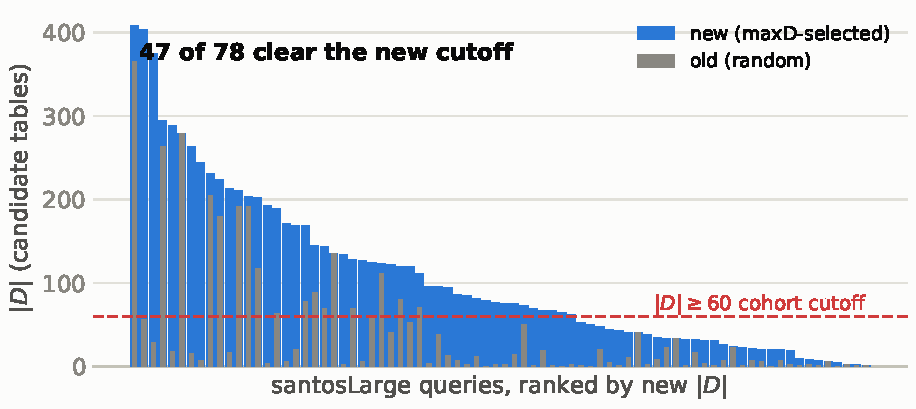
\includegraphics[width=\linewidth]{figures/sl_maxd_before_after.pdf}
\end{column}
\end{columns}
\vspace{4pt}
{\footnotesize\color{Muted} Instead of restricting to a thin 19-query tail, we re-picked \emph{which} attribute/value each query targets -- deliberately, not randomly -- so far more of the 78 queries carry a usable $|D|$. Methodology and the resulting cohort are the next two slides; every santosLarge slide after them uses that new cohort.}
\end{frame}

\begin{frame}{santosLarge: choosing attributes/values to maximize $|D|$}{Why random assignment fails, and what replaces it}
\textbf{Why the original (random) assignment gives small $|D|$}
\begin{itemize}\small
  \item Each query's protected attribute/value came from \texttt{starmie\_fair}'s \texttt{experimental\_setup.py} (\texttt{selection\_strategy='random'}, seed 42): pick a random categorical column, then \texttt{random.choice(unique\_values)} -- with no regard for how common that value is \emph{elsewhere} in the 11{,}086-table datalake.
  \item $|D|$ is driven entirely by cross-table value popularity (via the overlap posting-list) intersected with semantic column similarity -- a purely random value usually lands on something rare.
\end{itemize}
\vspace{4pt}
\textbf{The replacement: rank by a free proxy, verify by real retrieval}
\begin{itemize}\small
  \item Per query table: enumerate every (categorical attr, value) pair from its own synopsis (excluding the empty-cell bucket).
  \item Rank all candidates by \highlight{$|$postings$[$value$]|$} -- the overlap index's own posting-list size -- a free, no-retrieval proxy for "how many $(table,attr)$ pairs would pass the overlap filter."
  \item Verify the top 20 candidates by \emph{actual} retrieval ($\mathrm{top\_n}{=}5000$, same context every santosLarge script uses); keep whichever gives the single largest real $|D|$ -- \highlight{maximize, no target, no early exit}.
\end{itemize}
\vspace{4pt}
{\footnotesize\color{Muted} This is a deliberate, documented departure from the original random selection, not a bug fix -- see next: it systematically favors common/generic values over rare ones, which is exactly what makes $|D|$ large.}
\end{frame}

\begin{frame}{santosLarge: what changed, concretely}{Old (random) vs.\ new (maxD) assignment, three examples}
\small
\begin{tabular}{@{}p{0.30\textwidth}p{0.33\textwidth}p{0.33\textwidth}@{}}
\textbf{Table} & \textbf{Old: attr $\to$ value ($|D|$)} & \textbf{New: attr $\to$ value ($|D|$)} \\[2pt]
\texttt{cabinet-office...} & \texttt{Organisation} $\to$ \texttt{Cabinet Office} (17) & \texttt{Valid?} $\to$ \texttt{1} (213) \\[4pt]
\texttt{1004ipopayments.csv} & \texttt{Date} $\to$ \texttt{20/04/2010} (2) & \texttt{Expense type} $\to$ \texttt{Other} (134) \\[4pt]
\texttt{Dec\_19.csv} & (unnamed) $\to$ \texttt{09/12/2019} (6) & (unnamed) $\to$ \texttt{Entity} (171) \\
\end{tabular}
\vspace{8pt}

\highlight{The pattern is consistent}: new values skew heavily toward generic/structural tokens (\texttt{0}, \texttt{1.0}, \texttt{Headcount}, \texttt{Entity}, \texttt{Other}) rather than the specific, often-unique values random selection picked (a particular date, org name, or country). That is the mechanism behind the $|D|$ gain -- these are values that recur across many tables in this GOV.UK-style organizational-report corpus, not meaningfully rare "protected" attributes anymore.

\vspace{4pt}
{\footnotesize\color{Muted} A handful of tables ($\sim$4 of 78) improve little or not at all even after checking up to $\sim$200 candidates each (e.g.\ \texttt{biodiversity\_by\_county.csv}, $|D|{=}1\to1$) -- a genuine intrinsic limit (no other table is both semantically similar and value-overlapping), not a search-budget problem.}
\end{frame}

\begin{frame}{santosLarge: picking the $|D|$ threshold and $(k,\alpha)$ grid}{Data-driven, not carried over from the old grid}
\centering
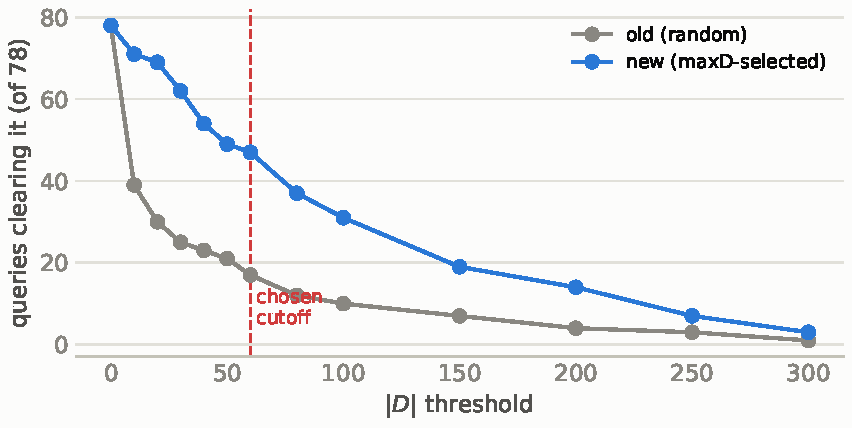
\includegraphics[width=0.78\linewidth]{figures/sl_maxd_threshold_curve.pdf}

\vspace{4pt}
\small\color{Ink2}
Old (random) $|D|$: median 11, max 365. New (maxD): median 77, mean 108, max 408. With the old grid ($k\in\{10,20\},\alpha\in\{2,3\}$, max pool $60$) carried over unexamined, the pool size would say nothing about the new distribution -- so the grid is re-derived from it instead: \highlight{$k\in\{10,15\},\ \alpha\in\{2,3,4\}$} (pool sizes 20--60) and cohort \highlight{$|D|\geq 60$}, chosen so every retained query stays \emph{unclamped across all six cells} -- one consistent, comparable population for the whole sweep, same design principle as the original cohort, recalibrated to the new distribution.

\vspace{2pt}
{\footnotesize\color{Muted} Result: \highlight{47 of 78} queries retained (vs.\ 19 of 78 before) -- the cohort every santosLarge slide after this one uses.}
\end{frame}

\begin{frame}{santosLarge: choosing $F^\star$, $\delta$, and $\tau$}{Reach-maximizing}
\centering
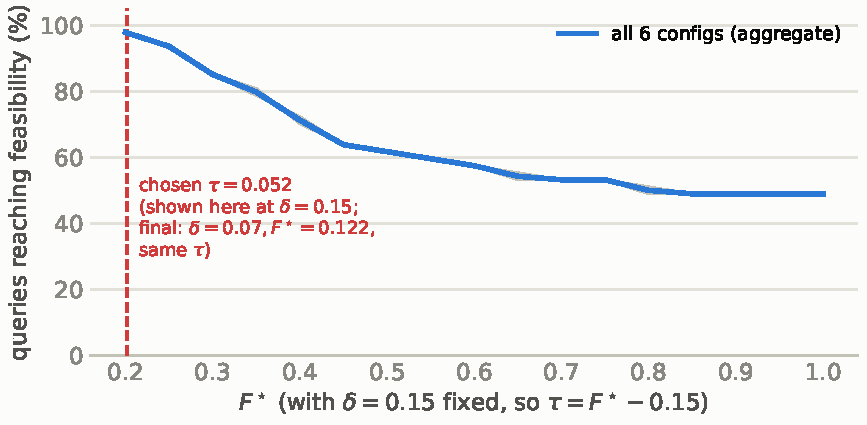
\includegraphics[width=0.66\linewidth]{figures/sl_tau_sweep_curve.pdf}

\vspace{2pt}
\footnotesize\color{Ink2}
Only $\tau=F^\star-\delta$ enters anything mechanically ($U$ -- hence $\delta$/$F^\star$ individually -- never appears in Stage 2's constraints, only its objective), so ``maximize reach'' with no floor trivially wants $\tau\to0$. We fixed $\delta$, swept $F^\star$ from the $\tau\geq0.05$ floor, and re-solved Stage 2 only across all $47\times6{=}282$ cells (candidates scored $U{=}1.0$ -- feasibility doesn't depend on $U$). \highlight{Reach is uniform across $\alpha$ at fixed $k$} -- $\alpha$ creates no bottleneck here.

\vspace{2pt}
santosLarge is the \emph{scalability} benchmark. $\delta{=}0.70$ (tried first) made the tolerance band nearly meaningless; tightened to \highlight{$\delta{=}0.07$}. For $\tau$: rather than sit at the floor, found the largest $\tau$ keeping every query feasible in every config -- breaks at $\tau{=}0.0533$ -- so used \highlight{$\tau{=}0.052,\ F^\star{=}0.122$}.

\vspace{2pt}
{\footnotesize\color{Muted} Sweep cohort: the same $n=47$, $|D|\geq60$ population as the previous slide. See \texttt{experiments/santoslarge\_tau\_sweep.py}.}
\end{frame}

\begin{frame}{santosLarge: one outlier, and why we exclude rather than relax}{Getting to 100\% honestly}
\small
\begin{itemize}
  \item At $\tau{=}0.05$: \highlight{46 of 47} queries reach feasibility in \emph{every} one of the 6 $(k,\alpha)$ cells -- 98\% overall (276/282), matching the previous slide.
  \item The entire gap is \highlight{one single query}: \texttt{SpendoverC2A3500Apr17.csv}, infeasible in all 6 of its configs at $\tau{=}0.05$ -- but feasible again at $\tau\leq0.03$. Its achievable $F$ (even after Stage 1's $\arg\max F$) sits just under the floor.
  \item \textbf{Two ways to reach 100\%}: lower the floor to $\tau{=}0.03$ for everyone (undoes the floor we deliberately set, to rescue one outlier), or \highlight{exclude that one query} and keep $\tau{=}0.05$.
\end{itemize}
\vspace{4pt}
\textbf{We exclude it (Option 3).} Lowering the floor to fix one outlier would mean the floor was never really a floor -- and it's a narrower, more honest exclusion than relaxing a constraint for the whole cohort. The remaining \highlight{$n=46$} queries reach exactly \highlight{100\%} feasibility (276/276) at $\tau{=}0.052,\ F^\star{=}0.122,\ \delta{=}0.07$ already chosen -- not a relaxed target, the one already agreed on.

\vspace{2pt}
{\footnotesize\color{Muted} Final cohort for every santosLarge slide from here on: $n{=}46$ ($|D|\geq60$, minus \texttt{SpendoverC2A3500Apr17.csv}) $\times\,6$ configs ($k\in\{10,15\},\alpha\in\{2,3,4\}$) $=276$ rows. See \texttt{experiments/santoslarge\_maxd\_study.py}.}
\end{frame}

\begin{frame}{santosLarge: one-off index cost}
\centering
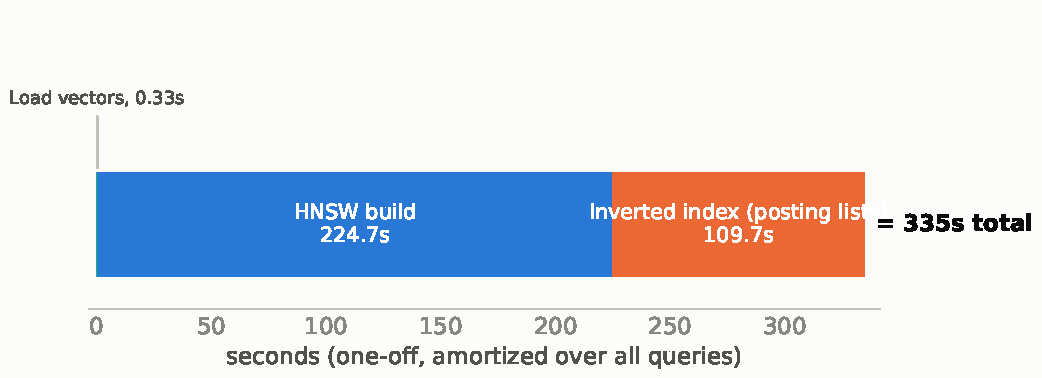
\includegraphics[width=0.95\linewidth]{figures/sl_index_build.pdf}

\vspace{6pt}
\small\color{Ink2}
The HNSW (semantic) index now dominates build cost (225--272s across two rebuilds), ahead of the posting-list (overlap) index at a stable 109--110s -- both read every one of 11{,}086 tables. \highlight{HNSW build time varies $\sim$21\% run-to-run} (the posting-list build does not): \texttt{hnswlib}'s multi-threaded \texttt{add\_items} makes graph construction order, and hence wall-clock cost, non-deterministic even with a fixed seed. On disk, the HNSW index (\highlight{281.8 MB}, 84{,}157 elements $\times$ 768 dims) is $\sim$17$\times$ larger than the posting-list index (\highlight{16.9 MB}, 277{,}704 distinct values). Amortized over all queries; not part of any per-query timing on the following slides.

\vspace{2pt}
{\footnotesize\color{Muted} One-off, over all 78 santosLarge queries -- built once, independent of the $n{=}46$ cohort used below.}
\end{frame}

\begin{frame}{santosLarge: $\alpha$ finally bites}
\centering
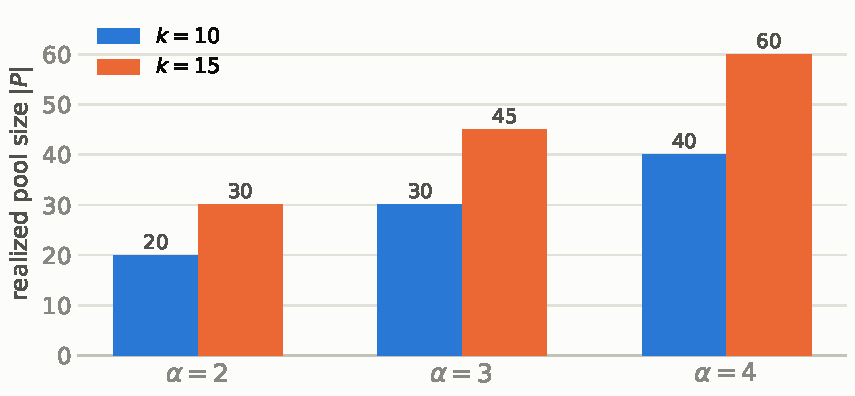
\includegraphics[width=0.7\linewidth]{figures/sl_pool_scaling.pdf}

\vspace{4pt}
\small\color{Ink2}
Realized pool size $|P|$ tracks the requested $\alpha k$ \highlight{exactly} (20 / 30 / 40 / 30 / 45 / 60) -- the C5 clamp fires on \highlight{0 of 276} rows here: the $|D|\geq60$ cohort was chosen specifically so no cell clamps.

\vspace{2pt}
{\footnotesize\color{Muted} Cohort: \highlight{$n=46$} per config, all feasible -- $P$ is built before Stage 2 runs, so this holds regardless of outcome (here, every row reaches $\tau$ anyway -- see the outcome slide two ahead).}
\end{frame}

\begin{frame}{santosLarge: per-stage time scales with $\alpha k$, not $|D|$}
\centering
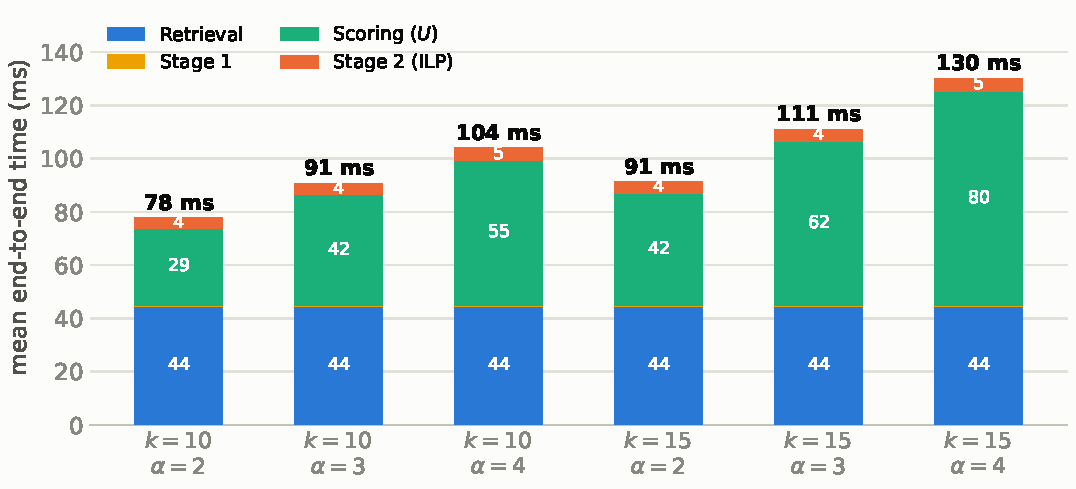
\includegraphics[width=0.8\linewidth]{figures/sl_stage_timing_scaling.pdf}

\vspace{2pt}
\small\color{Ink2}
\textbf{This is the efficiency claim, made visible.} Retrieval is flat (fixed cost of probing the index); \highlight{scoring grows with $\alpha k$} (roughly 20\,ms at $\alpha k{=}20$ up to over 100\,ms at $\alpha k{=}60$); Stage 1 stays under a tenth of a millisecond throughout, Stage 2 a few milliseconds.

{\footnotesize\color{Muted} Cohort: \highlight{$n=46$} per config, all feasible -- every query is timed the same way regardless of the (now uniformly positive) outcome.}
\end{frame}

\begin{frame}{santosLarge: outcome and Stage 1 convergence}
\centering
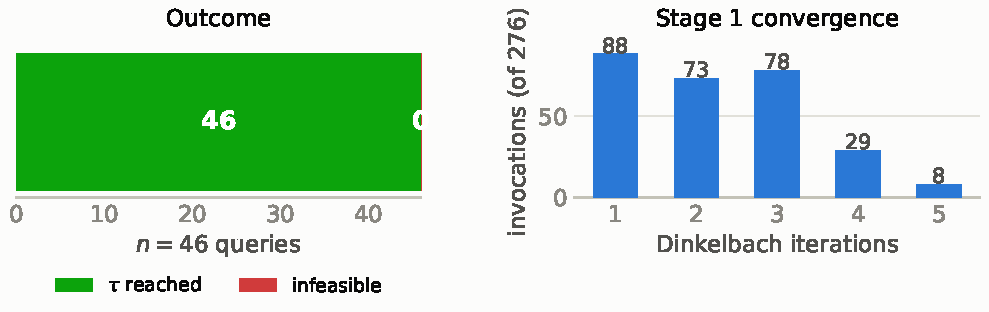
\includegraphics[width=0.92\linewidth]{figures/sl_outcome_dinkelbach.pdf}

\vspace{2pt}
\small\color{Ink2}
\highlight{All 46 of 46} queries reach $\tau$ in \emph{every} $(k,\alpha)$ cell -- by construction of the cohort (Option 3: the one query that didn't was excluded, not papered over with a lower floor). Dinkelbach runs on every row (never clamped) and converges in \highlight{1--5 iterations} (mean 2.3).

\vspace{2pt}
{\footnotesize\color{Muted} Cohort: \highlight{left panel, $n=46$} (one config shown -- 46 reach $\tau$, 0 don't, identically across all 6 configs); \highlight{right panel, $n=276$} Dinkelbach invocations out of 276 rows (46 queries $\times$ 6 configs) -- none are C5-clamped.}
\end{frame}

\begin{frame}{santosLarge: convergence time and iterations by pool size}{Mean per query, $n=46$ at each pool size}
\small
\begin{center}
\begin{tabular}{cccccc}
\toprule
$k$ & $\alpha$ & pool ($\alpha k$) & Stage 1 time & mean iters & range \\
\midrule
10 & 2 & 20 & 0.317\,ms & 2.11 & 1--5 \\
10 & 3 & 30 & 0.370\,ms & 2.26 & 1--5 \\
10 & 4 & 40 & 0.391\,ms & 2.43 & 1--5 \\
15 & 2 & 30 & 0.368\,ms & 2.26 & 1--5 \\
15 & 3 & 45 & 0.383\,ms & 2.30 & 1--5 \\
15 & 4 & 60 & 0.388\,ms & 2.20 & 1--5 \\
\bottomrule
\end{tabular}
\end{center}

\vspace{4pt}
\small\color{Ink2}
\highlight{Convergence time tracks pool size only weakly} -- 0.317\,ms at pool 20 to 0.391\,ms at pool 40, a $\sim$23\% rise for a $2\times$ larger pool -- since each iteration is one sort-and-select over the pool, not a re-scan proportional to some larger structure. \highlight{Iteration count doesn't increase monotonically with pool size at all} (pool 45's mean 2.30 exceeds pool 60's 2.20): convergence speed is a property of how skewed the pool's $N_i/n_i$ ratios are, not of how large the pool is.

\vspace{2pt}
{\footnotesize\color{Muted} Cohort: $n=46$ per row, all Dinkelbach invocations (none clamped). See \texttt{experiments/RESULTS-santoslarge.md} \S4 for the full breakdown.}
\end{frame}

\begin{frame}{santosLarge: convergence vs.\ \emph{input} pool size $|D|$}{Setting: $k{=}10,\alpha{=}3$ fixed (output pool $\alpha k{=}30$); \texttt{top\_n} swept from 5{,}000}
\footnotesize
\begin{center}
\begin{tabular}{ccccc}
\toprule
requested \texttt{top\_n} & actual mean $|D|$ & clamped & Stage 1 time & mean iters \\
\midrule
5{,}000 & 160.4 & 0/46 & 0.196\,ms & 2.26 \\
10{,}000 & 208.6 & 0/46 & 0.249\,ms & 2.22 \\
15{,}000 & 236.0 & 0/46 & 0.281\,ms & 2.26 \\
20{,}000 & 250.6 & 0/46 & 0.293\,ms & 2.28 \\
25{,}000 & 257.9 & 0/46 & 0.302\,ms & 2.28 \\
30{,}000 & 259.0 & 0/46 & 0.301\,ms & 2.28 \\
\bottomrule
\end{tabular}
\end{center}

\vspace{4pt}
\small\color{Ink2}
The previous slide varies the pool Stage 1 \emph{selects} ($\alpha k$) at fixed \texttt{top\_n}; this one fixes $k,\alpha$ and varies the pool Stage 1 \emph{searches over} ($|D|$) by sweeping \texttt{top\_n} -- \texttt{top\_n} is the dial, \highlight{realized $|D|$} is what's reported (yield $\ne$ \texttt{top\_n} after the overlap filter). Swept from $5{,}000$ since smaller \texttt{top\_n} clamps ($\alpha k{=}30\ge|D|$, $18/46$ at \texttt{top\_n}$=500$ in an earlier pass), so every point here is clamp-free. \highlight{Time scales with $|D|$} -- $\sim\!1.5\times$ from $|D|{\approx}160$ to $259$ -- one $O(|D|\log|D|)$ sort per iteration. \highlight{$|D|$ plateaus} past \texttt{top\_n}$\approx\!20{,}000$ ($+3\%$ over a $50\%$ larger \texttt{top\_n}) as the finite overlap-matching pool is exhausted, and time flattens in step. \highlight{Iteration count stays flat} (2.22--2.28): convergence takes only a few iterations regardless of search-pool size -- the $|D|$-dependence is in per-iteration sort cost, not iteration count.

\vspace{2pt}
{\footnotesize\color{Muted} Same 46-query cohort, re-retrieved per \texttt{top\_n}. Script: \texttt{experiments/santoslarge\_topn\_pool\_sweep.py}. See \texttt{experiments/RESULTS-santoslarge.md} \S4b.}
\end{frame}

\begin{frame}{santosLarge: precheck + actual solver only}{Excludes constraint-setup/verification overhead}
\footnotesize
\begin{center}
\begin{tabular}{ccccccc}
\toprule
$\alpha$ & $k$ & pool & LP precheck & MILP solver & precheck+solver & full Stage 2 \\
\midrule
2 & 10 & 20 & 0.677\,ms & 1.164\,ms & \textbf{1.842\,ms} & 2.055\,ms \\
2 & 15 & 30 & 0.677\,ms & 1.276\,ms & \textbf{1.953\,ms} & 2.160\,ms \\
3 & 10 & 30 & 0.654\,ms & 1.092\,ms & \textbf{1.745\,ms} & 1.946\,ms \\
3 & 15 & 45 & 0.757\,ms & 1.356\,ms & \textbf{2.112\,ms} & 2.337\,ms \\
4 & 10 & 40 & 0.679\,ms & 1.338\,ms & \textbf{2.017\,ms} & 2.224\,ms \\
4 & 15 & 60 & 0.783\,ms & 1.507\,ms & \textbf{2.291\,ms} & 2.518\,ms \\
\bottomrule
\end{tabular}
\end{center}

\vspace{4pt}
\small\color{Ink2}
"Full Stage 2" (§5) is precheck + \highlight{actual MILP solve} + constraint-setup/post-solve-verification overhead ($\sim$0.2--0.25\,ms, small and roughly constant). Isolating just the two solves: the \highlight{MILP solver dominates} ($\sim$60--65\% of precheck+solver time), the LP precheck the remaining $\sim$35--40\%, both growing mildly with pool size.

\vspace{2pt}
{\footnotesize\color{Muted} Caveat: absolute ms here differ from \S5's LP-time column for identical $(k,\alpha)$ cells -- sub-millisecond \texttt{perf\_counter} timings are noisy across process runs ($\pm$30\% or so); the relative split (solver $>$ precheck) is the stable finding. See \texttt{RESULTS-santoslarge.md} \S5c.}
\end{frame}

\begin{frame}{santosLarge: two-stage vs.\ skipping Stage 1}
\centering
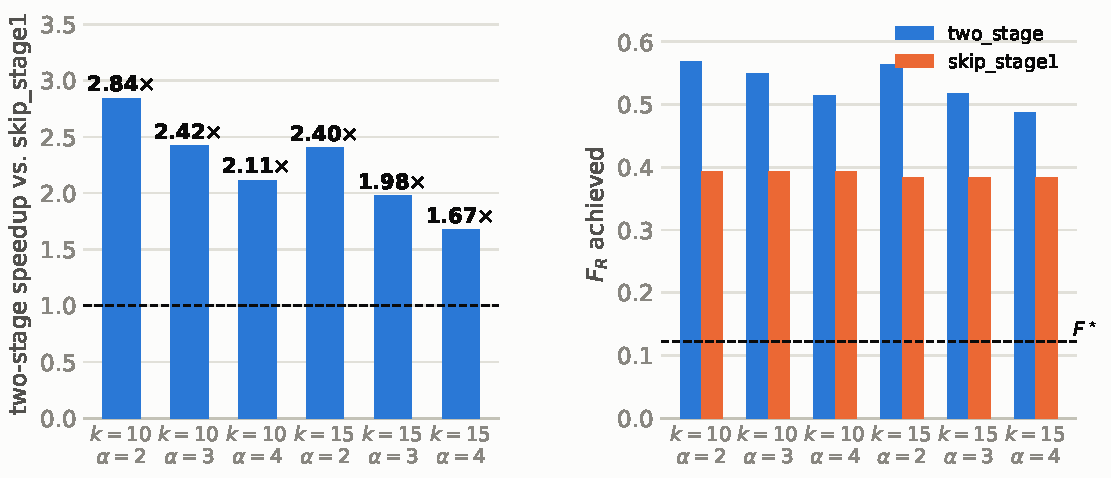
\includegraphics[width=0.86\linewidth]{figures/sl_skip_stage1.pdf}

\vspace{2pt}
\small\color{Ink2}
Stage 1 earns its place on \highlight{speed} (1.7--2.8$\times$ faster, growing with $\alpha k$) but costs \bad{$\Sigma U$}: skip\_stage1 optimizes over the superset $D\supseteq P$, so it can only match or beat two-stage there (roughly 5--9\% higher $\Sigma U$ here). Both satisfy $F_R\geq\tau$; $F_R$'s distance from $F^\star{=}0.122$ is a diagnostic, not a constraint either violates -- achieved $F_R$ sits around 0.49--0.57 on average (individual rows range 0.052--1.0), comfortably above $\tau{=}0.052$ and, on average, above $F^\star$ too, since neither stage targets $F^\star$ directly (C3) -- Stage 1's unbounded $\arg\max F$ pushes past it.

\vspace{2pt}
{\footnotesize\color{Muted} Cohort: \highlight{$n=46$} per config, all feasible in both arms (both left and right panels) -- unlike the original cohort, there's no feasible-only restriction needed here.}
\end{frame}

% ============================================================================
\section{WDC -- scalability at 50.8M-table scale}
% ============================================================================
\begin{frame}{WDC: a genuinely large, uncurated corpus}{50.8M web tables from Common Crawl -- \texttt{tier\_10k} and \texttt{tier\_100k}, \texttt{tier\_1m} pending}
\small
Unlike santos/santosLarge, WDC ships \highlight{no query/datalake split and no curated query list} -- query tables are drawn algorithmically, and (unlike santos-family benchmarks) \highlight{the set of query tables is not fixed}: any table that doesn't work out can simply be replaced.

\vspace{6pt}
\textbf{Critical constraint: \texttt{tier\_10k} $\subset$ \texttt{tier\_100k}} exactly (verified directly: all 10{,}001 \texttt{tier\_10k} files appear in \texttt{tier\_100k}) -- so a valid scale comparison must hold the \emph{same} query tables fixed across tiers and observe how the surrounding datalake's growth changes outcomes, not optimize a different query set per tier.

\vspace{6pt}
The old approach (superseded here) inflated $|D|$ by \bad{relaxing \S7.3's retrieval rule itself} ($D_{sem}\cup D_{ovl}$). This section replaces that with santosLarge's maxD methodology instead -- \S7.3-faithful intersection retrieval throughout, applied to a single shared query set.

{\footnotesize\color{Muted} Old union-mode report/figures backed up under \texttt{experiments/results/\_backup\_pre\_maxd\_wdc/}.}
\end{frame}

\begin{frame}{WDC: query selection -- one shared set, not per-tier}{Candidates drawn from \texttt{tier\_10k} only; maxD choice made using \texttt{tier\_100k}}
\small
\begin{enumerate}
  \item Candidates drawn from \texttt{tier\_10k}'s table universe only (guaranteed present in every larger nested tier).
  \item maxD attribute/value selection against the larger \texttt{tier\_100k} context (rank by free posting-list proxy, verify top 20 by real retrieval, keep the largest $|D|$).
  \item That fixed \texttt{(table,attr,value)} triple is evaluated for real $|D|$ against every tier's own index.
\end{enumerate}
\vspace{4pt}
{\footnotesize\color{Muted} \texttt{top\_n=5000}. \texttt{tier\_10k}$\subset$\texttt{tier\_100k}$\subset$\texttt{tier\_1m} nesting verified directly.}
\end{frame}

\begin{frame}{WDC: an unclamped-by-construction grid -- santosLarge rigor, applied here}{Revised after finding the original grid was 87\% clamped}
\small
An initial 30-cell grid ($k\in\{10..50\}\times\alpha\in\{10..60\}$, max pool 3{,}000) never required $|D|\geq\max(\alpha k)$ the way santosLarge's cohort did -- measured directly, \highlight{87.1\% of its 900 (query,cell) pairs were already clamped} at \texttt{top\_n=5000}. Reverted to santosLarge's discipline instead:

\vspace{4pt}
\begin{enumerate}
  \item Widen the candidate pool to \highlight{210} (60 original + 150 more, same seeded shuffle).
  \item Use $\min(D_{10k},D_{100k})$ as the binding threshold; derive the grid from the observed distribution: $k\in\{5,10,20\}\times\alpha\in\{5,10\}$ -- 6 cells, pools 25--200.
  \item Retain every candidate with $\min(D_{10k},D_{100k})\geq 200$ -- guaranteed unclamped on \emph{both} tiers, every cell.
\end{enumerate}
\vspace{4pt}
\highlight{67 of 210 retained (31.9\%)} -- comparable in spirit to santosLarge's 47/78.

{\footnotesize\color{Muted} \texttt{experiments/wdc/wdc\_maxd\_selection\_unclamped.py}; notes in \texttt{experiments/results/wdc\_unclamped\_selection\_notes.md}.}
\end{frame}

\begin{frame}{WDC: choosing $F^\star,\delta,\tau$ -- 100\% joint feasibility}{$\tau$ floor 0.05, same round values as before}
\small
Swept for \emph{joint} feasibility on the new 6-cell grid + 67-candidate pool: a query only counts if every one of its 6 cells is feasible on \emph{both} tiers simultaneously.

\vspace{6pt}
\textbf{Chosen: $F^\star{=}0.20$, $\delta{=}0.10$, $\tau{=}0.10$}:

\begin{center}
\begin{tabular}{lccc}
\toprule
& \texttt{tier\_10k} feasible & \texttt{tier\_100k} feasible & \textbf{feasible on BOTH} \\
\midrule
of 67 candidates & 67/67 & 67/67 & \textbf{67/67 (100\%)} \\
\bottomrule
\end{tabular}
\end{center}

\vspace{4pt}
\highlight{Every candidate that cleared the $|D|\geq 200$ threshold is also fully feasible} -- no outlier exclusion needed, unlike the original design.
\end{frame}

\begin{frame}{WDC: final query cohort -- 67 tables, identical across tiers}{100\% retention at the chosen threshold/grid}
\small
\textbf{All 67 query tables (same attribute, same value) used against every tier} -- no exclusions.

\vspace{6pt}
\begin{itemize}
  \item Threshold: $\min(D_{10k},D_{100k})\geq 200$, grid $k\in\{5,10,20\}\times\alpha\in\{5,10\}$ (max pool 200).
  \item All 67 feasible across all 6 grid cells, on \emph{both} tiers.
\end{itemize}

\vspace{6pt}
{\footnotesize\color{Muted} Final cohort: \texttt{experiments/results/wdc\_unclamped\_final\_cohort.csv}. \texttt{tier\_1m}'s embeddings/metadata store are built (\texttt{tier\_100k}$\subset$\texttt{tier\_1m} nesting verified) -- full end-to-end study on this 67-query cohort, all three tiers, still pending.}
\end{frame}


\begin{frame}{WDC: one-off index cost, all three tiers}{HNSW size scales linearly; build time does not scale uniformly}
\small
\begin{center}
\begin{tabular}{lrrrrr}
\toprule
tier & tables & HNSW build & HNSW size & inv.\ build & inv.\ size \\
\midrule
\texttt{tier\_10k} & 10{,}000 & 13.9\,s & 163.6\,MB & 2.7\,s & 8.75\,MB \\
\texttt{tier\_100k} & 100{,}000 & 200.8\,s & 1{,}633.0\,MB & 23.4\,s & 76.6\,MB \\
\texttt{tier\_1m} & 999{,}999 & 1{,}284.8\,s & 16{,}322.8\,MB & 49.6\,s & 670.5\,MB \\
\bottomrule
\end{tabular}
\end{center}

\vspace{6pt}
\highlight{HNSW size scales almost perfectly linearly} throughout (163.6\,MB $\to$ 1{,}633.0\,MB $\to$ 16{,}322.8\,MB -- $\sim$10$\times$ at every 10$\times$ step) -- expected, one fixed-size embedding per table regardless of scale. \highlight{HNSW build time scaling is NOT uniform}: $\sim$14.5$\times$ from \texttt{tier\_10k}$\to$\texttt{tier\_100k} (superlinear, $O(n\log n)$-consistent) but only $\sim$6.4$\times$ from \texttt{tier\_100k}$\to$\texttt{tier\_1m} (sublinear) -- not investigated further here, but a real, reported pattern rather than a single clean exponent. \highlight{Inverted-index vocabulary grows sublinearly at every step} (995{,}957 $\to$ 6{,}444{,}399 distinct values, $\sim$6.5$\times$ for $10\times$ tables): common values keep getting reused rather than each new table contributing an entirely new vocabulary.

\vspace{2pt}
{\footnotesize\color{Muted} Sizes are on-disk after native serialization (\texttt{hnswlib.save\_index}; pickled postings dict) -- neither index is persisted by the normal pipeline, both rebuilt in-memory on every \texttt{build\_wdc\_context} call. \texttt{tier\_1m} required a memory-frugal rewrite of the measurement script: this account has a hard 32GB per-process RSS limit (\texttt{ulimit -m}, confirmed non-adjustable), and the straightforward approach (keeping the raw vectors dict, its categorical-filtered copy, AND hnswlib's own internal copy alive at once) peaked near that ceiling and was twice silently killed. Script: \texttt{experiments/wdc/wdc\_index\_size\_report.py}.}
\end{frame}

\begin{frame}{HNSW size, explained: it's categorical columns, not tables}{santosLarge vs.\ all three WDC tiers -- same underlying constant}
\small
\texttt{HnswRetriever} only ever indexes \highlight{categorical columns} ($\theta_{\mathrm{cat}}{=}50$-bounded): \texttt{categorical\_only\_vectors} zeroes every non-categorical column's embedding before it reaches \texttt{hnswlib}, and \texttt{\_flatten} skips zero-norm rows -- so the indexed population matches the overlap index's exactly.

\vspace{4pt}
\begin{center}
\begin{tabular}{lrrrr}
\toprule
dataset & total cols & \textbf{cat.\ cols (indexed)} & HNSW size & bytes/elem \\
\midrule
santosLarge & 121{,}796 & 84{,}157 (69.1\%) & 281.78\,MB & 3{,}511.4 \\
\texttt{tier\_10k} & 51{,}854 & 48{,}857 (94.2\%) & 163.59\,MB & 3{,}512.0 \\
\texttt{tier\_100k} & 518{,}131 & 487{,}728 (94.1\%) & 1{,}633.02\,MB & 3{,}512.6 \\
\texttt{tier\_1m} & 5{,}177{,}216 & 4{,}874{,}987 (94.2\%) & 16{,}322.76\,MB & 3{,}512.1 \\
\bottomrule
\end{tabular}
\end{center}

\vspace{6pt}
\highlight{Bytes/element is a true constant, $\sim$3{,}512, across all four datasets} (768-dim float32 vector + \texttt{hnswlib} graph links at $M{=}32$) -- so index size is exactly (indexed elements) $\times$ (fixed per-element cost), nothing else. santosLarge's index is $\sim$58$\times$ smaller than \texttt{tier\_1m}'s purely because it has $\sim$58$\times$ fewer categorical columns (84{,}157 vs.\ 4{,}874{,}987) -- not because its tables are smaller (they aren't: santosLarge's are far \emph{bigger}, $\sim$5{,}000 rows vs.\ WDC's $\sim$6). \highlight{Coverage ratio explains why}: santosLarge's larger tables make $\theta_{\mathrm{cat}}{=}50$ a real, selective filter (69.1\%), while WDC's tiny tables (median $\sim$6 rows) mean \texttt{nunique(col)} is capped by row count itself, so almost every column qualifies as categorical (94.1--94.2\%, flat across all three tiers).

\vspace{2pt}
{\footnotesize\color{Muted} Total/categorical column counts computed directly from each tier's metadata store / \texttt{CsvSynopsis} (\texttt{experiments/context.py::column\_coverage\_stats}), $\theta_{\mathrm{cat}}{=}50$.}
\end{frame}

\begin{frame}{Inverted index size, explained: two different growth curves}{Not a fixed per-element cost like HNSW -- postings and vocabulary scale differently}
\footnotesize
\begin{center}
\begin{tabular}{lrrrrr}
\toprule
dataset & cat.\ cols & distinct vals & postings & avg dom/col & avg fan-out \\
\midrule
santosLarge & 84{,}157 & 277{,}704 & 887{,}428 & 10.54 & 3.20 \\
\texttt{tier\_10k} & 48{,}857 & 141{,}737 & 329{,}064 & 6.74 & 2.32 \\
\texttt{tier\_100k} & 487{,}728 & 995{,}957 & 3{,}347{,}443 & 6.86 & 3.36 \\
\texttt{tier\_1m} & 4{,}874{,}987 & 6{,}444{,}399 & 33{,}453{,}833 & 6.86 & 5.19 \\
\bottomrule
\end{tabular}
\end{center}

\vspace{6pt}
\highlight{Total postings tracks categorical-column count almost exactly linearly} (avg domain size/column is flat per dataset: $\sim$10.5 for santosLarge, $\sim$6.7--6.9 for WDC, capped by WDC's $\sim$6-row median table size, not corpus scale) -- this is why postings grow $\sim$10$\times$ per 10$\times$ WDC tables, matching column-count growth. \highlight{Vocabulary (distinct values) grows sub-linearly instead}: common web-table values (``1'', ``yes'', country names, \ldots) keep getting reused rather than each new table contributing new ones, so \highlight{average fan-out climbs with scale} (2.32 $\to$ 3.36 $\to$ 5.19) -- the same value attaches to more \texttt{(table,attr)} pairs as WDC grows.

\vspace{4pt}
Size itself is a \bad{pickle-framing proxy, not a native format} (unlike HNSW's \texttt{save\_index}) -- bytes/posting stays roughly stable ($\sim$20--28, pickle memoizes repeated table-name strings) but \highlight{bytes/distinct-value rises with scale} (63.7 $\to$ 64.7 $\to$ 80.6 $\to$ 109.1) since each key's \texttt{Set} payload grows with fan-out. Net effect: \texttt{tier\_1m}'s inverted index is $\sim$40$\times$ larger than santosLarge's (670.45\,MB vs.\ 16.86\,MB) -- smaller than the $\sim$58$\times$ column-count gap, because WDC's lower avg domain/column partly offsets its far larger column count.

\vspace{2pt}
{\footnotesize\color{Muted} avg dom/col = postings/cat.\ cols; avg fan-out = postings/distinct values. Same source data as the previous slide's inverted-index sizes.}
\end{frame}

\begin{frame}{WDC: Dinkelbach convergence vs.\ input pool size, all three tiers}{$k{=}20,\alpha{=}10$ (pool$=200$, the grid's own ceiling) -- 67-query cohort, all 6 top\_n values}
\tiny
\begin{center}
\begin{tabular}{lrrrrrr}
\toprule
tier & top\_n & mean $|D|$ & n\_ran & n\_clamped & mean stage-1 & mean iters \\
\midrule
\texttt{tier\_10k} & 5{,}000 & 387.0 & 67 & 0 & 0.67\,ms & 2.16 \\
\texttt{tier\_10k} & 10{,}000 & 618.4 & 67 & 0 & 1.26\,ms & 2.48 \\
\texttt{tier\_10k} & 15{,}000 & 776.2 & 67 & 0 & 1.53\,ms & 2.48 \\
\texttt{tier\_10k} & 20{,}000 & 854.1 & 67 & 0 & 1.72\,ms & 2.57 \\
\texttt{tier\_10k} & 25{,}000 & 877.9 & 67 & 0 & 1.80\,ms & 2.57 \\
\texttt{tier\_10k} & 30{,}000 & 882.6 & 67 & 0 & 1.88\,ms & 2.58 \\
\texttt{tier\_100k} & 5{,}000 & 925.5 & 67 & 0 & 1.45\,ms & 1.99 \\
\texttt{tier\_100k} & 10{,}000 & 1{,}409.1 & 67 & 0 & 2.25\,ms & 2.22 \\
\texttt{tier\_100k} & 15{,}000 & 1{,}755.3 & 67 & 0 & 3.30\,ms & 2.31 \\
\texttt{tier\_100k} & 20{,}000 & 2{,}048.0 & 67 & 0 & 4.08\,ms & 2.37 \\
\texttt{tier\_100k} & 25{,}000 & 2{,}371.9 & 67 & 0 & 5.33\,ms & 2.42 \\
\texttt{tier\_100k} & 30{,}000 & 2{,}630.7 & 67 & 0 & 6.44\,ms & 2.51 \\
\texttt{tier\_1m} & 5{,}000 & 1{,}338.7 & 62 & 5 & 2.17\,ms & 1.58 \\
\texttt{tier\_1m} & 10{,}000 & 2{,}629.7 & 66 & 1 & 4.82\,ms & 1.77 \\
\texttt{tier\_1m} & 15{,}000 & 3{,}440.9 & 65 & 2 & 6.77\,ms & 1.85 \\
\texttt{tier\_1m} & 20{,}000 & 4{,}215.8 & 66 & 1 & 7.87\,ms & 1.88 \\
\texttt{tier\_1m} & 25{,}000 & 4{,}971.4 & 65 & 2 & 11.04\,ms & 1.86 \\
\texttt{tier\_1m} & 30{,}000 & 5{,}633.9 & 65 & 2 & 11.56\,ms & 1.97 \\
\bottomrule
\end{tabular}
\end{center}

\vspace{4pt}
\footnotesize
\highlight{Iteration count stays essentially flat (1.58--2.58) across three orders of magnitude of corpus size}, direct empirical support for the paper's ``converges in only a few iterations'' claim (\S5). \highlight{Stage-1 time tracks $|D|$, not $|T|$} and stays under 12\,ms everywhere. \highlight{Clamping is essentially absent at this grid's own ceiling}: 0/67 on \texttt{tier\_10k}/\texttt{tier\_100k}, only 1--5/67 on \texttt{tier\_1m} (mild non-monotonicity, not a bug).

\vspace{2pt}
{\footnotesize\color{Muted} \texttt{tier\_1m}'s context required a batched-\texttt{add\_items} HNSW build plus $M{=}16$ (vs.\ $M{=}32$ elsewhere) to fit this account's 32GB RSS ceiling -- a memory-driven exception, not a scalability finding; index now cached to disk. Script: \texttt{experiments/wdc/wdc\_topn\_pool\_sweep.py}.}
\end{frame}

\begin{frame}{WDC: Dinkelbach convergence at a second grid cell -- $k{=}10,\alpha{=}3$ (pool$=30$)}{Same 67-query cohort, same top\_n sweep -- a smaller, easier pool}
\tiny
\begin{center}
\begin{tabular}{lrrrrrr}
\toprule
tier & top\_n & mean $|D|$ & n\_ran & n\_clamped & mean stage-1 & mean iters \\
\midrule
\texttt{tier\_10k} & 5{,}000 & 387.0 & 67 & 0 & 0.54\,ms & 2.06 \\
\texttt{tier\_10k} & 10{,}000 & 618.3 & 67 & 0 & 0.87\,ms & 1.94 \\
\texttt{tier\_10k} & 15{,}000 & 775.7 & 67 & 0 & 1.11\,ms & 2.00 \\
\texttt{tier\_10k} & 20{,}000 & 853.3 & 67 & 0 & 1.21\,ms & 1.93 \\
\texttt{tier\_10k} & 25{,}000 & 877.2 & 67 & 0 & 1.23\,ms & 1.93 \\
\texttt{tier\_10k} & 30{,}000 & 881.9 & 67 & 0 & 1.27\,ms & 1.93 \\
\texttt{tier\_100k} & 5{,}000 & 807.9 & 67 & 0 & 1.31\,ms & 1.76 \\
\texttt{tier\_100k} & 10{,}000 & 1{,}289.4 & 67 & 0 & 1.90\,ms & 1.75 \\
\texttt{tier\_100k} & 15{,}000 & 1{,}571.3 & 67 & 0 & 2.12\,ms & 1.66 \\
\texttt{tier\_100k} & 20{,}000 & 1{,}847.5 & 67 & 0 & 2.47\,ms & 1.73 \\
\texttt{tier\_100k} & 25{,}000 & 2{,}111.3 & 67 & 0 & 3.63\,ms & 1.75 \\
\texttt{tier\_100k} & 30{,}000 & 2{,}368.6 & 67 & 0 & 3.54\,ms & 1.70 \\
\texttt{tier\_1m} & 5{,}000 & 1{,}071.4 & 66 & 1 & 1.42\,ms & 1.47 \\
\texttt{tier\_1m} & 10{,}000 & 1{,}898.0 & 66 & 1 & 2.81\,ms & 1.48 \\
\texttt{tier\_1m} & 15{,}000 & 2{,}840.6 & 66 & 1 & 4.90\,ms & 1.61 \\
\texttt{tier\_1m} & 20{,}000 & 3{,}559.3 & 66 & 1 & 6.13\,ms & 1.52 \\
\texttt{tier\_1m} & 25{,}000 & 4{,}355.4 & 66 & 1 & 7.61\,ms & 1.52 \\
\texttt{tier\_1m} & 30{,}000 & 5{,}133.4 & 66 & 1 & 10.57\,ms & 1.61 \\
\bottomrule
\end{tabular}
\end{center}

\vspace{3pt}
\footnotesize
\highlight{Same qualitative findings, more strongly}: mean iterations are lower still (1.47--2.06 vs.\ 1.58--2.58) -- a smaller pool is a cheaper top-$k$ selection. \highlight{Clamping is even rarer}: 0/67 on \texttt{tier\_10k}/\texttt{tier\_100k}, a consistent 1/67 on \texttt{tier\_1m} at every \texttt{top\_n}.

\vspace{1pt}
{\footnotesize\color{Muted} \texttt{tier\_1m} loaded its index from the previous slide's disk cache (seconds, not $\sim$14\,min). Caveat: \texttt{tier\_100k}'s mean $|D|$ differs slightly from the previous slide's despite retrieval not depending on $k/\alpha$ -- hnswlib's multi-threaded build is seed-deterministic in its own choices but not concurrent insertion order, so independent rebuilds over identical data can differ slightly. Full data: \texttt{wdc\_topn\_pool\_sweep\_k10\_a3.csv}.}
\end{frame}

\begin{frame}{WDC: Stage 2 execution time -- LP pre-check vs.\ MILP solver, all three tiers}{top\_n$=5000$, $\alpha\in\{10,5\}\times k\in\{5,10,20\}$, 67-query cohort -- WDC analogue of santosLarge \S5c}
\tiny
\begin{center}
\begin{tabular}{lrrrrrrrrr}
\toprule
tier & $\alpha$ & $k$ & pool & clamped & feasible & LP precheck & MILP solver & \textbf{pre+solver} & full wall \\
\midrule
\texttt{tier\_10k} & 10 & 5 & 50 & 0 & 67/67 & 1.071\,ms & 1.583\,ms & \textbf{2.654\,ms} & 2.905\,ms \\
\texttt{tier\_10k} & 10 & 10 & 100 & 0 & 67/67 & 0.994\,ms & 1.697\,ms & \textbf{2.691\,ms} & 2.938\,ms \\
\texttt{tier\_10k} & 10 & 20 & 200 & 0 & 67/67 & 1.202\,ms & 2.162\,ms & \textbf{3.364\,ms} & 3.651\,ms \\
\texttt{tier\_10k} & 5 & 5 & 25 & 0 & 67/67 & 0.873\,ms & 1.426\,ms & \textbf{2.299\,ms} & 2.530\,ms \\
\texttt{tier\_10k} & 5 & 10 & 50 & 0 & 67/67 & 0.891\,ms & 1.467\,ms & \textbf{2.359\,ms} & 2.593\,ms \\
\texttt{tier\_10k} & 5 & 20 & 100 & 0 & 67/67 & 0.980\,ms & 1.677\,ms & \textbf{2.658\,ms} & 2.905\,ms \\
\texttt{tier\_100k} & 10 & 5 & 50 & 0 & 67/67 & 1.183\,ms & 2.148\,ms & \textbf{3.331\,ms} & 3.625\,ms \\
\texttt{tier\_100k} & 10 & 10 & 100 & 0 & 67/67 & 1.181\,ms & 2.887\,ms & \textbf{4.068\,ms} & 4.364\,ms \\
\texttt{tier\_100k} & 10 & 20 & 200 & 0 & 67/67 & 1.376\,ms & 4.341\,ms & \textbf{5.717\,ms} & 6.048\,ms \\
\texttt{tier\_100k} & 5 & 5 & 25 & 0 & 67/67 & 0.992\,ms & 2.322\,ms & \textbf{3.314\,ms} & 3.583\,ms \\
\texttt{tier\_100k} & 5 & 10 & 50 & 0 & 67/67 & 1.019\,ms & 2.122\,ms & \textbf{3.141\,ms} & 3.421\,ms \\
\texttt{tier\_100k} & 5 & 20 & 100 & 0 & 67/67 & 1.135\,ms & 3.221\,ms & \textbf{4.357\,ms} & 4.648\,ms \\
\texttt{tier\_1m} & 10 & 5 & 50 & 1 & 60/67 & 1.682\,ms & 2.153\,ms & \textbf{3.835\,ms} & 3.912\,ms \\
\texttt{tier\_1m} & 10 & 10 & 100 & 1 & 60/67 & 1.201\,ms & 2.210\,ms & \textbf{3.411\,ms} & 3.449\,ms \\
\texttt{tier\_1m} & 10 & 20 & 200 & 4 & 60/67 & 1.354\,ms & 2.705\,ms & \textbf{4.059\,ms} & 4.073\,ms \\
\texttt{tier\_1m} & 5 & 5 & 25 & 1 & 60/67 & 0.976\,ms & 1.706\,ms & \textbf{2.682\,ms} & 2.746\,ms \\
\texttt{tier\_1m} & 5 & 10 & 50 & 1 & 60/67 & 0.990\,ms & 1.812\,ms & \textbf{2.802\,ms} & 2.860\,ms \\
\texttt{tier\_1m} & 5 & 20 & 100 & 1 & 60/67 & 1.086\,ms & 1.962\,ms & \textbf{3.048\,ms} & 3.098\,ms \\
\bottomrule
\end{tabular}
\end{center}

\vspace{3pt}
\footnotesize
\highlight{Stage 2 is a few ms everywhere} (2.3--6.0\,ms), growing $\sim$1.5--1.7$\times$ for an 8$\times$ larger pool and only $\sim$1.4$\times$ for 100$\times$ more tables; the MILP is $\sim$55--76\% of pre+solver. \highlight{New at \texttt{tier\_1m}: the LP pre-check becomes decisive} -- 7/67 queries are LP-infeasible at every cell (MILP skipped), since the cohort's $\tau$ was validated only on the two smaller tiers.

\vspace{1pt}
{\footnotesize\color{Muted} $U$ is seeded synthetic uniform(0,1), not real unionability (\texttt{tier\_1m}'s lean context has no full vectors dict); retrieval re-run per tier, so $|D|$ is not bit-identical to earlier slides for the smaller tiers; \texttt{tier\_1m} uses the cached $M{=}16$ index. LP averaged over all rows, MILP over LP-feasible rows only. Script: \texttt{wdc\_stage2\_timing.py}.}
\end{frame}

\begin{frame}{WDC \texttt{tier\_1m}: what the LP pre-check saves on the 7 infeasible queries}{MILP skipped when the LP proves infeasibility -- measured by re-running those 7 pools with and without the pre-check}
\small
\begin{center}
\begin{tabular}{rrrrrr}
\toprule
$\alpha$ & $k$ & pool & with pre-check & MILP only (no pre-check) & saved / query \\
\midrule
10 & 20 & 200 & 1.004\,ms & 1.102\,ms & 0.098\,ms \\
10 & 10 & 100 & 0.862\,ms & 1.096\,ms & 0.234\,ms \\
10 & 5 & 50 & 0.895\,ms & 1.133\,ms & 0.238\,ms \\
5 & 20 & 100 & 0.839\,ms & 1.033\,ms & 0.194\,ms \\
5 & 10 & 50 & 0.763\,ms & 1.005\,ms & 0.242\,ms \\
5 & 5 & 25 & 0.738\,ms & 1.015\,ms & 0.277\,ms \\
\bottomrule
\end{tabular}
\end{center}

\vspace{6pt}
\highlight{The saving is small: $\sim$0.1--0.28\,ms per skipped query, $\sim$0.7--1.9\,ms across all 7.} HiGHS also detects infeasibility quickly on its own, so skipping the MILP avoids $\sim$1\,ms of work while the LP itself costs $\sim$0.7--0.9\,ms -- at these pool sizes the pre-check is close to break-even. Its value here is soundness and avoiding branch-and-bound on harder instances, which these pools are not.

\vspace{2pt}
{\footnotesize\color{Muted} Median of 5 in-process repetitions per pool, warm caches, so absolute values are lower than the previous slide's means (which include cold runs and feasible rows); treat as $\pm$30\%. Both variants returned infeasible on every pool. Same seeded synthetic $U$ and $\tau{=}0.10$ as the previous slide.}
\end{frame}

\begin{frame}{WDC: per-stage and end-to-end time, real unionability, all three tiers}{top\_n$=5000$, $\alpha\in\{10,5\}\times k\in\{5,10,20\}$, 67-query cohort -- mean ms}
\tiny
\begin{center}
\setlength{\tabcolsep}{3pt}
\begin{tabular}{lrrrrrrrrrrrr}
\toprule
tier & $\alpha$ & $k$ & pool & clamp & feas. & retrieval & Stage 1 & \textbf{unionab.} & LP & MILP & Stage 2 & \textbf{end-to-end} \\
\midrule
\texttt{tier\_10k} & 10 & 5 & 50 & 0 & 67/67 & 15.9 & 0.62 & 12.83 & 1.57 & 2.23 & 4.05 & \textbf{33.4} \\
\texttt{tier\_10k} & 10 & 10 & 100 & 0 & 67/67 & 15.9 & 0.89 & 24.96 & 1.27 & 2.22 & 3.73 & \textbf{45.4} \\
\texttt{tier\_10k} & 10 & 20 & 200 & 0 & 67/67 & 15.9 & 0.98 & 45.94 & 1.53 & 2.81 & 4.62 & \textbf{67.4} \\
\texttt{tier\_10k} & 5 & 5 & 25 & 0 & 67/67 & 15.9 & 0.93 & 8.28 & 1.02 & 1.85 & 3.08 & \textbf{28.2} \\
\texttt{tier\_10k} & 5 & 10 & 50 & 0 & 67/67 & 15.9 & 0.79 & 13.85 & 1.05 & 1.98 & 3.25 & \textbf{33.7} \\
\texttt{tier\_10k} & 5 & 20 & 100 & 0 & 67/67 & 15.9 & 0.88 & 25.06 & 1.19 & 2.21 & 3.64 & \textbf{45.4} \\
\texttt{tier\_100k} & 10 & 5 & 50 & 0 & 67/67 & 33.0 & 1.19 & 12.55 & 1.57 & 2.26 & 4.09 & \textbf{50.8} \\
\texttt{tier\_100k} & 10 & 10 & 100 & 0 & 67/67 & 33.0 & 1.76 & 26.69 & 1.28 & 2.43 & 3.96 & \textbf{65.4} \\
\texttt{tier\_100k} & 10 & 20 & 200 & 0 & 67/67 & 33.0 & 1.85 & 49.08 & 1.44 & 2.96 & 4.67 & \textbf{88.6} \\
\texttt{tier\_100k} & 5 & 5 & 25 & 0 & 67/67 & 33.0 & 1.75 & 7.66 & 0.99 & 1.85 & 3.05 & \textbf{45.5} \\
\texttt{tier\_100k} & 5 & 10 & 50 & 0 & 67/67 & 33.0 & 1.61 & 13.14 & 0.98 & 1.88 & 3.08 & \textbf{50.8} \\
\texttt{tier\_100k} & 5 & 20 & 100 & 0 & 67/67 & 33.0 & 1.70 & 25.35 & 1.18 & 2.28 & 3.70 & \textbf{63.8} \\
\texttt{tier\_1m} & 10 & 5 & 50 & 1 & 60/67 & 351.3 & 1.46 & 11.71 & 2.14 & 3.42 & 5.48 & \textbf{370.0} \\
\texttt{tier\_1m} & 10 & 10 & 100 & 1 & 60/67 & 351.3 & 2.07 & 24.52 & 1.27 & 2.37 & 3.62 & \textbf{381.5} \\
\texttt{tier\_1m} & 10 & 20 & 200 & 4 & 60/67 & 351.3 & 2.07 & 46.01 & 1.41 & 5.40 & 6.49 & \textbf{405.9} \\
\texttt{tier\_1m} & 5 & 5 & 25 & 1 & 60/67 & 351.3 & 1.99 & 7.03 & 1.01 & 1.86 & 2.86 & \textbf{363.2} \\
\texttt{tier\_1m} & 5 & 10 & 50 & 1 & 60/67 & 351.3 & 1.93 & 12.68 & 1.01 & 1.94 & 2.95 & \textbf{368.9} \\
\texttt{tier\_1m} & 5 & 20 & 100 & 1 & 60/67 & 351.3 & 1.95 & 24.12 & 1.15 & 2.58 & 3.66 & \textbf{381.1} \\
\bottomrule
\end{tabular}
\end{center}

\vspace{3pt}
\footnotesize
\highlight{Retrieval is the only stage that grows with the corpus}: 15.9 $\to$ 33.0 $\to$ 351.3\,ms per query, 86--97\% of end-to-end on \texttt{tier\_1m}. \highlight{Unionability scoring is linear in the pool, independent of the corpus}: $\sim$0.23--0.26\,ms per pool table on every tier (200 tables: 45.9 / 49.1 / 46.0\,ms) -- the $\alpha k$ efficiency claim, measured. Stage 1 (0.6--2.1\,ms) and Stage 2 (2.9--6.5\,ms) stay small and scale-free.

\vspace{1pt}
{\footnotesize\color{Muted} Real pinned-match $U$ ($\sigma{=}0.6$), supersedes the synthetic-$U$ Stage 2 slide. Retrieval (HNSW probe + overlap filter + $N_i/n_i$ lookup) is independent of $k,\alpha$ and timed once per query. \texttt{tier\_1m}: cached $M{=}16$ index, peak RSS $\approx$31.8\,GiB of the 32\,GiB cap (tight). MILP averaged over LP-feasible rows. Details: \texttt{wdc-report.md} \S5.}
\end{frame}

\begin{frame}{WDC: why \texttt{tier\_1m} retrieval is slow -- HNSW vs.\ overlap probe}{top\_n$=5000$, 67-query cohort, mean per query; retrieval = HNSW probe + overlap probe + join + $N_i/n_i$ lookup}
\footnotesize
\begin{center}
\setlength{\tabcolsep}{4pt}
\begin{tabular}{lrrrrrrr}
\toprule
tier & HNSW probe (ms) & overlap probe (ms) & join (ms) & lookup (ms) & \textbf{total (ms)} & $|D_{ovl}|$ & $|D|$ \\
\midrule
\texttt{tier\_10k}  & 8.1  & 1.2   & 1.0  & 1.2 & \textbf{11.4}  & 3{,}289   & 388 \\
\texttt{tier\_100k} & 9.3  & 15.5  & 2.1  & 2.9 & \textbf{29.9}  & 34{,}038  & 888 \\
\texttt{tier\_1m}   & 10.2 & 203.5 & 24.4 & 3.6 & \textbf{241.7} & 341{,}014 & 1{,}071 \\
\bottomrule
\end{tabular}
\end{center}
\vspace{3pt}
\highlight{The HNSW probe is almost flat} (8.1 $\to$ 9.3 $\to$ 10.2\,ms for 100$\times$ more tables). \highlight{The overlap probe is the cause}: it returns every (table, column) pair containing the protected value, and that set grows $\sim$10$\times$ per tier (3.3k $\to$ 34k $\to$ 341k), so its time grows $\sim$13$\times$ then $\sim$13$\times$ (1.2 $\to$ 15.5 $\to$ 203.5\,ms) -- 84\% of \texttt{tier\_1m} retrieval. The join (dict + set intersection over those pairs) grows the same way (24.4\,ms at 1M). Only $\sim$1{,}000 pairs survive the intersection, so almost all of the overlap work is thrown away.

\vspace{1pt}
{\footnotesize\color{Muted} Same query grid and cached indexes as the previous slide; repeating each probe immediately gives nearly the same time (HNSW 8.6\,ms, overlap 196\,ms at 1M), so this is not cold-cache or paging cost. Totals (241.7\,ms) are lower than the 351\,ms above because this run had no 32\,GiB memory cap (peak 46\,GiB), so the two are different machine conditions; the split is the finding. Details: \texttt{wdc-report.md} \S5.1.}
\end{frame}

\begin{frame}{Benefit of Stage 1: post-retrieval pipeline time}{top\_n$=30000$, $k{=}10$, $\alpha{=}3$ (pool $\alpha k{=}30$) -- mean ms per query, timed from just before Stage 1 to the end of the pipeline}
\footnotesize
\begin{center}
\setlength{\tabcolsep}{3pt}
\begin{tabular}{lrr rrrr rrr rr}
\toprule
& & & \multicolumn{4}{c}{Two-stage (scores $\alpha k{=}30$)} & \multicolumn{3}{c}{Stage 1 skipped (scores $|D|$)} & \multicolumn{2}{c}{Saving} \\
\cmidrule(lr){4-7}\cmidrule(lr){8-10}\cmidrule(lr){11-12}
Dataset & $n$ & $|D|$ & S1 & score & S2 & \textbf{total} & score & S2 & \textbf{total} & \% & $\times$ \\
\midrule
Santos-Large & 46 & 259 & 0.29 & 39.68 & 3.18 & \textbf{43.2} & 386.5 & 4.0 & \textbf{390.5} & \textbf{88.9} & 9.0 \\
WDC-10K & 67 & 881 & 1.33 & 9.21 & 2.10 & \textbf{12.6} & 227.9 & 10.5 & \textbf{238.4} & \textbf{94.7} & 18.9 \\
WDC-100K & 67 & 2518 & 3.49 & 7.06 & 2.84 & \textbf{13.4} & 433.0 & 36.9 & \textbf{470.0} & \textbf{97.1} & 35.1 \\
WDC-1M & 66 & 5211 & 8.82 & 6.46 & 4.85 & \textbf{20.1} & 667.3 & 525.8 & \textbf{1193.1} & \textbf{98.3} & 59.3 \\
\bottomrule
\end{tabular}
\end{center}
\vspace{3pt}
\footnotesize
Same retrieved $D$ in both conditions, so they differ only in whether Stage 1 runs. \highlight{Two-stage} = Stage 1 (Dinkelbach) $\to$ score $U$ on the 30-table pool $\to$ Stage 2 over the pool. \highlight{Stage 1 skipped} = score $U$ on all of $D$ $\to$ Stage 2 over $D$ at cardinality $k$. Saving $=(T_{\text{skip}}-T_{\text{two}})/T_{\text{skip}}$.

\vspace{1pt}
{\footnotesize\color{Muted} Retrieval, the overlap intersection and the $N_i/n_i$ lookup are outside the timed window (identical in both). $F^\star/\delta$: $0.122/0.07$ on Santos-Large, $0.20/0.10$ on the WDC tiers. HNSW indexes are cached to disk, so $|D|$ is reproducible across runs. One WDC-1M query has $|D|{=}2<k$ and is excluded. Details: \texttt{stage1-benefit-report.md}.}
\end{frame}

\begin{frame}{What the Stage 1 table shows}{In plain terms}
\footnotesize
\begin{itemize}
  \item \highlight{The bigger the data lake, the more Stage 1 saves}: 88.9\% on Santos-Large, 94.7\% on WDC-10K, 97.1\% on WDC-100K, 98.3\% on WDC-1M (9.0$\times$ to 59.3$\times$). Stage 1 caps unionability computations at $\alpha k = 30$ no matter how many candidates retrieval returns, so the larger $|D|$ grows, the more work it removes.
  \item \highlight{Almost all of the saving is unionability scoring} -- 386.5\,ms $\to$ 39.7\,ms on Santos-Large, 667.3\,ms $\to$ 6.5\,ms on WDC-1M. That is 30 bipartite matchings instead of $|D|$ of them: the $\alpha k$-not-$|\mathcal{T}|$ claim, measured.
  \item \highlight{At WDC-1M, skipping Stage 1 also makes Stage 2 expensive}: its ILP runs over $\sim$5{,}211 candidates instead of 30, costing 525.8\,ms against 4.8\,ms. Both the scoring and the solving inflate, not just the scoring.
  \item \highlight{Stage 1 is nearly free}: 0.29--8.8\,ms, against savings of hundreds of ms.
  \item \highlight{Feasibility is unaffected} -- 46/46, 67/67, 67/67, 64/66, identical in both conditions. The distribution-aware pre-filter never cost a feasible answer here.
  \item \highlight{But the speedup is not free in quality}: the pool reaches 80--91\% of the $\Sigma U$ that scoring every candidate achieves. Stage 1 can exclude a high-$U$ table that Stage 2 would otherwise have chosen.
\end{itemize}

\vspace{1pt}
{\footnotesize\color{Muted} Absolute ms vary with machine load between runs (the same cached $|D|$ gave 181.8 and 238.9\,ms for WDC-10K's skip condition); the \emph{ratio} is the stable quantity. $|D|$ is right-skewed on WDC-1M (mean 5{,}211, median $\approx$3{,}557, max 16{,}715), so the median per-query saving there is 97.7\% against a mean of 98.3\%. $top\_n{=}30000$ is the deepest retrieval setting and so the largest $|D|$; the saving narrows at smaller $top\_n$.}
\end{frame}





% ============================================================================
\section{Takeaways}
% ============================================================================
\begin{frame}{Takeaways}
\footnotesize
\begin{itemize}
  \item The pipeline has \textbf{four} short-circuit points -- two before Stage 1 even runs (\texttt{insufficient\_candidates}, the C5 clamp), two around Stage 2 (LP-decisive, \texttt{stage2\_infeasible}).
  \vspace{2pt}
  \item \textbf{santosLarge} (redesigned: attributes/values deliberately chosen to maximize $|D|$, $|D|\geq 60$ cohort, $F^\star{=}0.122/\delta{=}0.07/\tau{=}0.052$ chosen to maximize reach without a degenerate $\tau$): the pipeline shows scoring cost scaling with $\alpha k$, Stage 1 buying a real 1.7--2.8$\times$ speedup at a 5--9\% $\Sigma U$ cost, and (unlike the original random-assignment cohort, where the LP pre-check was decisive on 37\% of instances) every one of the 46 retained queries is feasible in all 6 configs, so the LP pre-check has nothing left to catch here either.
  \vspace{2pt}
  \item \textbf{WDC, all three tiers} (redesigned, replacing the old $D_{sem}\cup D_{ovl}$ relaxation): santosLarge's maxD attribute/value selection, applied under \S7.3-faithful intersection retrieval to \highlight{the same query tables at every scale} ($\texttt{tier\_10k}\subset\texttt{tier\_100k}\subset\texttt{tier\_1m}$, verified) -- not independently-optimized per-tier cohorts. An initial 30-cell grid proved 87.1\% clamped; reverted to a santosLarge-style unclamped-by-construction 6-cell grid ($k\in\{5,10,20\}\times\alpha\in\{5,10\}$, max pool 200) over a widened 210-candidate pool, with $F^\star{=}0.20/\delta{=}0.10/\tau{=}0.10$ ($\tau$ floor 0.05) achieving \highlight{100\% joint feasibility (67/67)} on both tiers simultaneously. At $k{=}20,\alpha{=}10$ (pool$=200$), Dinkelbach converges in 1.58--2.58 mean iterations and under 12\,ms mean Stage-1 time \highlight{across all three tiers, three orders of magnitude of table count} -- clamping is essentially absent (0/67 on \texttt{tier\_10k}/\texttt{tier\_100k}, 1--5/67 on \texttt{tier\_1m}, a mild non-monotonicity effect, not a bug).
  \vspace{2pt}
  \item \textbf{Together}: santosLarge answers "does the two-stage design's efficiency claim hold when it has room to matter?"; WDC (all three tiers, redesigned cohort) confirms it does on an uncurated corpus too, at genuine million-table scale.
\end{itemize}
\end{frame}

\end{document}
